% Options for packages loaded elsewhere
\PassOptionsToPackage{unicode}{hyperref}
\PassOptionsToPackage{hyphens}{url}
\PassOptionsToPackage{dvipsnames,svgnames,x11names}{xcolor}
%
\documentclass[
  letterpaper,
  DIV=11,
  numbers=noendperiod]{scrartcl}

\usepackage{amsmath,amssymb}
\usepackage{iftex}
\ifPDFTeX
  \usepackage[T1]{fontenc}
  \usepackage[utf8]{inputenc}
  \usepackage{textcomp} % provide euro and other symbols
\else % if luatex or xetex
  \usepackage{unicode-math}
  \defaultfontfeatures{Scale=MatchLowercase}
  \defaultfontfeatures[\rmfamily]{Ligatures=TeX,Scale=1}
\fi
\usepackage{lmodern}
\ifPDFTeX\else  
    % xetex/luatex font selection
\fi
% Use upquote if available, for straight quotes in verbatim environments
\IfFileExists{upquote.sty}{\usepackage{upquote}}{}
\IfFileExists{microtype.sty}{% use microtype if available
  \usepackage[]{microtype}
  \UseMicrotypeSet[protrusion]{basicmath} % disable protrusion for tt fonts
}{}
\makeatletter
\@ifundefined{KOMAClassName}{% if non-KOMA class
  \IfFileExists{parskip.sty}{%
    \usepackage{parskip}
  }{% else
    \setlength{\parindent}{0pt}
    \setlength{\parskip}{6pt plus 2pt minus 1pt}}
}{% if KOMA class
  \KOMAoptions{parskip=half}}
\makeatother
\usepackage{xcolor}
\ifLuaTeX
  \usepackage{luacolor}
  \usepackage[soul]{lua-ul}
\else
  \usepackage{soul}
  
\fi
\setlength{\emergencystretch}{3em} % prevent overfull lines
\setcounter{secnumdepth}{-\maxdimen} % remove section numbering
% Make \paragraph and \subparagraph free-standing
\makeatletter
\ifx\paragraph\undefined\else
  \let\oldparagraph\paragraph
  \renewcommand{\paragraph}{
    \@ifstar
      \xxxParagraphStar
      \xxxParagraphNoStar
  }
  \newcommand{\xxxParagraphStar}[1]{\oldparagraph*{#1}\mbox{}}
  \newcommand{\xxxParagraphNoStar}[1]{\oldparagraph{#1}\mbox{}}
\fi
\ifx\subparagraph\undefined\else
  \let\oldsubparagraph\subparagraph
  \renewcommand{\subparagraph}{
    \@ifstar
      \xxxSubParagraphStar
      \xxxSubParagraphNoStar
  }
  \newcommand{\xxxSubParagraphStar}[1]{\oldsubparagraph*{#1}\mbox{}}
  \newcommand{\xxxSubParagraphNoStar}[1]{\oldsubparagraph{#1}\mbox{}}
\fi
\makeatother

\usepackage{color}
\usepackage{fancyvrb}
\newcommand{\VerbBar}{|}
\newcommand{\VERB}{\Verb[commandchars=\\\{\}]}
\DefineVerbatimEnvironment{Highlighting}{Verbatim}{commandchars=\\\{\}}
% Add ',fontsize=\small' for more characters per line
\usepackage{framed}
\definecolor{shadecolor}{RGB}{241,243,245}
\newenvironment{Shaded}{\begin{snugshade}}{\end{snugshade}}
\newcommand{\AlertTok}[1]{\textcolor[rgb]{0.68,0.00,0.00}{#1}}
\newcommand{\AnnotationTok}[1]{\textcolor[rgb]{0.37,0.37,0.37}{#1}}
\newcommand{\AttributeTok}[1]{\textcolor[rgb]{0.40,0.45,0.13}{#1}}
\newcommand{\BaseNTok}[1]{\textcolor[rgb]{0.68,0.00,0.00}{#1}}
\newcommand{\BuiltInTok}[1]{\textcolor[rgb]{0.00,0.23,0.31}{#1}}
\newcommand{\CharTok}[1]{\textcolor[rgb]{0.13,0.47,0.30}{#1}}
\newcommand{\CommentTok}[1]{\textcolor[rgb]{0.37,0.37,0.37}{#1}}
\newcommand{\CommentVarTok}[1]{\textcolor[rgb]{0.37,0.37,0.37}{\textit{#1}}}
\newcommand{\ConstantTok}[1]{\textcolor[rgb]{0.56,0.35,0.01}{#1}}
\newcommand{\ControlFlowTok}[1]{\textcolor[rgb]{0.00,0.23,0.31}{\textbf{#1}}}
\newcommand{\DataTypeTok}[1]{\textcolor[rgb]{0.68,0.00,0.00}{#1}}
\newcommand{\DecValTok}[1]{\textcolor[rgb]{0.68,0.00,0.00}{#1}}
\newcommand{\DocumentationTok}[1]{\textcolor[rgb]{0.37,0.37,0.37}{\textit{#1}}}
\newcommand{\ErrorTok}[1]{\textcolor[rgb]{0.68,0.00,0.00}{#1}}
\newcommand{\ExtensionTok}[1]{\textcolor[rgb]{0.00,0.23,0.31}{#1}}
\newcommand{\FloatTok}[1]{\textcolor[rgb]{0.68,0.00,0.00}{#1}}
\newcommand{\FunctionTok}[1]{\textcolor[rgb]{0.28,0.35,0.67}{#1}}
\newcommand{\ImportTok}[1]{\textcolor[rgb]{0.00,0.46,0.62}{#1}}
\newcommand{\InformationTok}[1]{\textcolor[rgb]{0.37,0.37,0.37}{#1}}
\newcommand{\KeywordTok}[1]{\textcolor[rgb]{0.00,0.23,0.31}{\textbf{#1}}}
\newcommand{\NormalTok}[1]{\textcolor[rgb]{0.00,0.23,0.31}{#1}}
\newcommand{\OperatorTok}[1]{\textcolor[rgb]{0.37,0.37,0.37}{#1}}
\newcommand{\OtherTok}[1]{\textcolor[rgb]{0.00,0.23,0.31}{#1}}
\newcommand{\PreprocessorTok}[1]{\textcolor[rgb]{0.68,0.00,0.00}{#1}}
\newcommand{\RegionMarkerTok}[1]{\textcolor[rgb]{0.00,0.23,0.31}{#1}}
\newcommand{\SpecialCharTok}[1]{\textcolor[rgb]{0.37,0.37,0.37}{#1}}
\newcommand{\SpecialStringTok}[1]{\textcolor[rgb]{0.13,0.47,0.30}{#1}}
\newcommand{\StringTok}[1]{\textcolor[rgb]{0.13,0.47,0.30}{#1}}
\newcommand{\VariableTok}[1]{\textcolor[rgb]{0.07,0.07,0.07}{#1}}
\newcommand{\VerbatimStringTok}[1]{\textcolor[rgb]{0.13,0.47,0.30}{#1}}
\newcommand{\WarningTok}[1]{\textcolor[rgb]{0.37,0.37,0.37}{\textit{#1}}}

\providecommand{\tightlist}{%
  \setlength{\itemsep}{0pt}\setlength{\parskip}{0pt}}\usepackage{longtable,booktabs,array}
\usepackage{calc} % for calculating minipage widths
% Correct order of tables after \paragraph or \subparagraph
\usepackage{etoolbox}
\makeatletter
\patchcmd\longtable{\par}{\if@noskipsec\mbox{}\fi\par}{}{}
\makeatother
% Allow footnotes in longtable head/foot
\IfFileExists{footnotehyper.sty}{\usepackage{footnotehyper}}{\usepackage{footnote}}
\makesavenoteenv{longtable}
\usepackage{graphicx}
\makeatletter
\newsavebox\pandoc@box
\newcommand*\pandocbounded[1]{% scales image to fit in text height/width
  \sbox\pandoc@box{#1}%
  \Gscale@div\@tempa{\textheight}{\dimexpr\ht\pandoc@box+\dp\pandoc@box\relax}%
  \Gscale@div\@tempb{\linewidth}{\wd\pandoc@box}%
  \ifdim\@tempb\p@<\@tempa\p@\let\@tempa\@tempb\fi% select the smaller of both
  \ifdim\@tempa\p@<\p@\scalebox{\@tempa}{\usebox\pandoc@box}%
  \else\usebox{\pandoc@box}%
  \fi%
}
% Set default figure placement to htbp
\def\fps@figure{htbp}
\makeatother

\KOMAoption{captions}{tableheading}
\makeatletter
\@ifpackageloaded{tcolorbox}{}{\usepackage[skins,breakable]{tcolorbox}}
\@ifpackageloaded{fontawesome5}{}{\usepackage{fontawesome5}}
\definecolor{quarto-callout-color}{HTML}{909090}
\definecolor{quarto-callout-note-color}{HTML}{0758E5}
\definecolor{quarto-callout-important-color}{HTML}{CC1914}
\definecolor{quarto-callout-warning-color}{HTML}{EB9113}
\definecolor{quarto-callout-tip-color}{HTML}{00A047}
\definecolor{quarto-callout-caution-color}{HTML}{FC5300}
\definecolor{quarto-callout-color-frame}{HTML}{acacac}
\definecolor{quarto-callout-note-color-frame}{HTML}{4582ec}
\definecolor{quarto-callout-important-color-frame}{HTML}{d9534f}
\definecolor{quarto-callout-warning-color-frame}{HTML}{f0ad4e}
\definecolor{quarto-callout-tip-color-frame}{HTML}{02b875}
\definecolor{quarto-callout-caution-color-frame}{HTML}{fd7e14}
\makeatother
\makeatletter
\@ifpackageloaded{caption}{}{\usepackage{caption}}
\AtBeginDocument{%
\ifdefined\contentsname
  \renewcommand*\contentsname{Table of contents}
\else
  \newcommand\contentsname{Table of contents}
\fi
\ifdefined\listfigurename
  \renewcommand*\listfigurename{List of Figures}
\else
  \newcommand\listfigurename{List of Figures}
\fi
\ifdefined\listtablename
  \renewcommand*\listtablename{List of Tables}
\else
  \newcommand\listtablename{List of Tables}
\fi
\ifdefined\figurename
  \renewcommand*\figurename{Figure}
\else
  \newcommand\figurename{Figure}
\fi
\ifdefined\tablename
  \renewcommand*\tablename{Table}
\else
  \newcommand\tablename{Table}
\fi
}
\@ifpackageloaded{float}{}{\usepackage{float}}
\floatstyle{ruled}
\@ifundefined{c@chapter}{\newfloat{codelisting}{h}{lop}}{\newfloat{codelisting}{h}{lop}[chapter]}
\floatname{codelisting}{Listing}
\newcommand*\listoflistings{\listof{codelisting}{List of Listings}}
\makeatother
\makeatletter
\makeatother
\makeatletter
\@ifpackageloaded{caption}{}{\usepackage{caption}}
\@ifpackageloaded{subcaption}{}{\usepackage{subcaption}}
\makeatother

\usepackage{bookmark}

\IfFileExists{xurl.sty}{\usepackage{xurl}}{} % add URL line breaks if available
\urlstyle{same} % disable monospaced font for URLs
\hypersetup{
  pdftitle={Beyond the Exclamation Points!!!},
  pdfauthor={Shachar Hochman},
  colorlinks=true,
  linkcolor={blue},
  filecolor={Maroon},
  citecolor={Blue},
  urlcolor={Blue},
  pdfcreator={LaTeX via pandoc}}


\title{Beyond the Exclamation Points!!!}
\usepackage{etoolbox}
\makeatletter
\providecommand{\subtitle}[1]{% add subtitle to \maketitle
  \apptocmd{\@title}{\par {\large #1 \par}}{}{}
}
\makeatother
\subtitle{HDI-ROPE for Binary Outcomes: What Makes a Text Message Spam?}
\author{Shachar Hochman}
\date{2025-05-21}

\begin{document}
\maketitle


\subsection{Why Are We Here?}\label{why-are-we-here}

\textbf{Goal}: Demonstrate a clearer approach to interpreting logistic
regression using Bayesian methods and HDI-ROPE analysis, illustrated
through real-world SMS spam detection.

\textbf{Case Study}: Predicting whether an SMS message is spam based on
linguistic toxicity patterns (captured through NLP+PCA), message length,
and punctuation usage.

\textbf{The Bottom Line}: This tutorial shows how Bayesian modeling
combined with marginal effects and HDI-ROPE analysis creates a more
intuitive workflow for binary outcome analysis---avoiding the notorious
``log-odds'' interpretation problem while tackling the practical
challenge of spam detection.

\begin{tcolorbox}[enhanced jigsaw, coltitle=black, colframe=quarto-callout-caution-color-frame, breakable, leftrule=.75mm, colbacktitle=quarto-callout-caution-color!10!white, bottomtitle=1mm, toprule=.15mm, titlerule=0mm, rightrule=.15mm, title=\textcolor{quarto-callout-caution-color}{\faFire}\hspace{0.5em}{I make assumptions (too)!}, arc=.35mm, opacitybacktitle=0.6, colback=white, left=2mm, toptitle=1mm, opacityback=0, bottomrule=.15mm]

I assume you:

- Have basic familiarity with R and the tidyverse.

- Understand the fundamentals of regression analysis.

- Have encountered logistic regression before and familiar with the
interpretation frustration.

\end{tcolorbox}

\subsection{The Messages Behind the Data: Understanding SMS Spam in
Context}\label{the-messages-behind-the-data-understanding-sms-spam-in-context}

Imagine receiving a text message: \textgreater{} ``URGENT!!! You have
WON £1,000,000!!! Reply NOW with your bank details!!!''

Your brain instantly recognizes this as spam---but how? It's not just
excessive exclamation points or too-good-to-be-true offers. There's a
complex pattern of linguistic signals distinguishing legitimate messages
from spam, which can vary significantly across cultural and linguistic
contexts.

The dataset we're exploring comes from the
\href{https://www.kaggle.com/datasets/ysfbil/exais-sms-dataset}{ExAIS
SMS Spam project} conducted in Nigeria, featuring 5,240 SMS messages
(2,350 spam, 2,890 ham) collected from university community members aged
20--50.

The data contain the SPAM/HAM (not spam) classification and the text
message itself. Using NLP magic, dimensionality reduction, and text
analysis (see note below for full code), I extracted some additional
features:

\begin{itemize}
\item
  \textbf{is\_spam} - Our outcome variable; a binary classification
  indicating spam or legitimate communication.
\item
  \textbf{pc\_aggression \& pc\_incoherence} - Principal components I
  extracted from Google's Perspective API toxicity scores capturing
  sophisticated linguistic patterns:

  \begin{itemize}
  \item
    \textbf{pc\_aggression:} threatening, toxic, and insulting language
    patterns..
  \item
    \textbf{pc\_incoherence} inflammatory, incoherent, or unsubstantial
    messages.
  \end{itemize}
\item
  \textbf{word\_count} - The total number of words per message (includes
  squared term to capture non-linear relationships).
\item
  \textbf{exclamation\_count} - The number of exclamation points, a
  simple but telling spam feature.
\end{itemize}

\ul{Our central question is this}: How do linguistic toxicity patterns
(captured by PCA components) interact with message characteristics like
length and punctuation to identify spam? And more importantly, how can
we interpret these relationships meaningfully?

\begin{tcolorbox}[enhanced jigsaw, coltitle=black, colframe=quarto-callout-note-color-frame, breakable, leftrule=.75mm, colbacktitle=quarto-callout-note-color!10!white, bottomtitle=1mm, toprule=.15mm, titlerule=0mm, rightrule=.15mm, title=\textcolor{quarto-callout-note-color}{\faInfo}\hspace{0.5em}{A Note on Advanced NLP Features}, arc=.35mm, opacitybacktitle=0.6, colback=white, left=2mm, toptitle=1mm, opacityback=0, bottomrule=.15mm]

Below is the exact, reproducible pipeline I used to transform raw text
into the two tidy principal‑component dials (\texttt{pc\_aggression},
\texttt{pc\_incoherence}) you saw in the main post. Everything is
wrapped in code‑chunks so you (or your future self) can copy‑paste the
whole block into \textbf{Quarto/R Markdown} and run it end‑to‑end.

\begin{Shaded}
\begin{Highlighting}[]
\CommentTok{\# ── 1 · Load required packages ───────────────────────────────────────────}
\FunctionTok{library}\NormalTok{(tidyverse)     }\CommentTok{\# data manipulation and pipes}
\FunctionTok{library}\NormalTok{(peRspective)   }\CommentTok{\# R client for Google/Jigsaw Perspective API}
\FunctionTok{library}\NormalTok{(FactoMineR)    }\CommentTok{\# Principal‑Component Analysis}
\FunctionTok{library}\NormalTok{(pROC)          }\CommentTok{\# ROC curves (for later evaluation)}
\end{Highlighting}
\end{Shaded}

\begin{quote}
\textbf{What is \emph{peRspective}?}\\
\texttt{peRspective} is a thin, tidyverse‑friendly wrapper around the
\href{https://developers.perspectiveapi.com/}{Perspective API}. It takes
care of batching requests, retrying on rate‑limits, and returning scores
as a clean data frame. Before running the chunk below you'll need a free
API key (set it once with
\texttt{Sys.setenv(PERSPECTIVE\_API\_KEY\ =\ "\textless{}your‑key\textgreater{}")}).
\end{quote}

\subsubsection{Step 1 -- Obtain linguistic scores from the Perspective
API}\label{step-1-obtain-linguistic-scores-from-the-perspective-api}

Each message is sent to the API, which returns up to nine probabilities
indicating the presence of attributes such as \emph{toxicity},
\emph{threat}, or \emph{incoherence}.

\begin{Shaded}
\begin{Highlighting}[]
\CommentTok{\# ⚠️  Disabled by default to avoid accidental quota use.}
\NormalTok{perspective\_scores }\OtherTok{\textless{}{-}}\NormalTok{ dataset\_clean }\SpecialCharTok{\%\textgreater{}\%}
  \FunctionTok{prsp\_stream}\NormalTok{(}
    \AttributeTok{text        =}\NormalTok{ message,          }\CommentTok{\# column containing the SMS text}
    \AttributeTok{text\_id     =}\NormalTok{ text\_id,          }\CommentTok{\# unique identifier for safe joins}
    \AttributeTok{score\_model =} \FunctionTok{c}\NormalTok{(}\StringTok{"THREAT"}\NormalTok{, }\StringTok{"TOXICITY"}\NormalTok{, }\StringTok{"INSULT"}\NormalTok{, }\StringTok{"SPAM"}\NormalTok{,}
                    \StringTok{"INFLAMMATORY"}\NormalTok{, }\StringTok{"INCOHERENT"}\NormalTok{, }\StringTok{"UNSUBSTANTIAL"}\NormalTok{,}
                    \StringTok{"FLIRTATION"}\NormalTok{, }\StringTok{"PROFANITY"}\NormalTok{),}
    \AttributeTok{safe\_output =} \ConstantTok{TRUE}\NormalTok{,             }\CommentTok{\# masks content the API flags as unsafe}
    \AttributeTok{verbose     =} \ConstantTok{TRUE}\NormalTok{)             }\CommentTok{\# progress messages}
\end{Highlighting}
\end{Shaded}

\begin{quote}
\textbf{Development tip:}\\
When iterating on downstream scripts, save the scores once
(\texttt{write\_csv()}) and reload them to avoid repeated network calls:

\begin{Shaded}
\begin{Highlighting}[]
\NormalTok{perspective\_scores }\OtherTok{\textless{}{-}} \FunctionTok{read\_csv}\NormalTok{(}\StringTok{"\textasciitilde{}/perspective\_scores\_saved.csv"}\NormalTok{)}
\end{Highlighting}
\end{Shaded}
\end{quote}

\subsubsection{Step 2 -- Merge, clean, and prepare for
PCA}\label{step-2-merge-clean-and-prepare-for-pca}

Occasionally a request fails or returns \texttt{NA}. We drop the few
problematic rows and replace any missing attribute scores with zeros so
PCA receives a complete numeric matrix.

\begin{Shaded}
\begin{Highlighting}[]
\NormalTok{scored\_data }\OtherTok{\textless{}{-}}\NormalTok{ dataset\_clean }\SpecialCharTok{\%\textgreater{}\%}
  \FunctionTok{left\_join}\NormalTok{(perspective\_scores, }\AttributeTok{by =} \StringTok{"text\_id"}\NormalTok{) }\SpecialCharTok{\%\textgreater{}\%}
  \FunctionTok{filter}\NormalTok{(}\SpecialCharTok{!}\NormalTok{(}\AttributeTok{has\_error =}\NormalTok{ (}\SpecialCharTok{!}\FunctionTok{is.na}\NormalTok{(error) }\SpecialCharTok{\&}\NormalTok{ error }\SpecialCharTok{!=} \StringTok{"No Error"}\NormalTok{))) }\SpecialCharTok{\%\textgreater{}\%}
  \FunctionTok{mutate}\NormalTok{(}\FunctionTok{across}\NormalTok{(THREAT}\SpecialCharTok{:}\NormalTok{PROFANITY, }\SpecialCharTok{\textasciitilde{}}\FunctionTok{replace\_na}\NormalTok{(.x, }\DecValTok{0}\NormalTok{))) }\SpecialCharTok{\%\textgreater{}\%}
  \FunctionTok{select}\NormalTok{(}\SpecialCharTok{{-}}\NormalTok{SPAM, }\SpecialCharTok{{-}}\NormalTok{FLIRTATION)   }\CommentTok{\# remove two attributes found redundant here}
\end{Highlighting}
\end{Shaded}

\subsubsection{Step 3 -- Reduce nine correlated scores to two principal
components}\label{step-3-reduce-nine-correlated-scores-to-two-principal-components}

Principal‑Component Analysis (PCA) rotates the nine‑dimensional
attribute space until the first component captures the largest
systematic variation, the second captures the next‑largest, and so on.

\begin{Shaded}
\begin{Highlighting}[]
\NormalTok{pca\_result }\OtherTok{\textless{}{-}} \FunctionTok{PCA}\NormalTok{(scored\_data }\SpecialCharTok{\%\textgreater{}\%} \FunctionTok{select}\NormalTok{(THREAT}\SpecialCharTok{:}\NormalTok{PROFANITY),}
                  \AttributeTok{ncp   =} \DecValTok{3}\NormalTok{,    }\CommentTok{\# keep three components for inspection}
                  \AttributeTok{graph =} \ConstantTok{FALSE}\NormalTok{)}

\NormalTok{pca\_scores }\OtherTok{\textless{}{-}} \FunctionTok{as\_tibble}\NormalTok{(pca\_result}\SpecialCharTok{$}\NormalTok{ind}\SpecialCharTok{$}\NormalTok{coord) }\SpecialCharTok{\%\textgreater{}\%}
  \FunctionTok{set\_names}\NormalTok{(}\FunctionTok{c}\NormalTok{(}\StringTok{"pc\_aggression"}\NormalTok{,     }\CommentTok{\# roughly: threat + toxicity + insult}
              \StringTok{"pc\_inflammatory"}\NormalTok{,   }\CommentTok{\# moderate mix (not used later)}
              \StringTok{"pc\_incoherence"}\NormalTok{)) }\SpecialCharTok{\%\textgreater{}\%}   \CommentTok{\# roughly: incoherent + unsubstantial}
  \FunctionTok{mutate}\NormalTok{(}\AttributeTok{text\_id =}\NormalTok{ scored\_data}\SpecialCharTok{$}\NormalTok{text\_id)}
\end{Highlighting}
\end{Shaded}

\begin{itemize}
\tightlist
\item
  \textbf{\texttt{pc\_aggression}} ranges from \emph{neutral tone} to
  \emph{overt hostility}.
\item
  \textbf{\texttt{pc\_incoherence}} tracks the continuum from
  \emph{cohesive message} to \emph{nonsensical or fragmentary text}.
\end{itemize}

These two components retain ≈ 72 \% of the total variance in the
original nine attributes, providing a compact yet informative
description of each message.

\subsubsection{Step 4 -- Assemble the modelling
table}\label{step-4-assemble-the-modelling-table}

Finally, we merge the PCA scores back with the pre‑computed surface
features (\texttt{word\_count}, \texttt{exclamation\_count}, etc.) so
the eventual model can consider both \textbf{linguistic tone} and
\textbf{formatting cues}.

\begin{Shaded}
\begin{Highlighting}[]
\NormalTok{model\_data }\OtherTok{\textless{}{-}}\NormalTok{ scored\_data }\SpecialCharTok{\%\textgreater{}\%}
  \FunctionTok{select}\NormalTok{(}\SpecialCharTok{{-}}\NormalTok{THREAT}\SpecialCharTok{:{-}}\NormalTok{PROFANITY) }\SpecialCharTok{\%\textgreater{}\%}
  \FunctionTok{left\_join}\NormalTok{(pca\_scores, }\AttributeTok{by =} \StringTok{"text\_id"}\NormalTok{)}
\end{Highlighting}
\end{Shaded}

At this point \texttt{model\_data} is a tidy, analysis‑ready data frame:
one row per SMS, interpretable columns for tone and structure, and no
missing values to trip up downstream methods.

\end{tcolorbox}

\subsection{\texorpdfstring{The Interpretation Challenge: Why Binary
Outcomes Are
Tricky}{The Interpretation Challenge:   Why Binary Outcomes Are Tricky}}\label{the-interpretation-challenge-why-binary-outcomes-are-tricky}

Logistic regression is the go-to tool when predicting binary
outcomes---spam vs.~legitimate, click vs.~no-click, win vs.~loss. But
before we dive into logistic regression, let's understand why ordinary
linear regression fails with binary data:

\subsubsection{Why a Simple Straight Line
Fails}\label{why-a-simple-straight-line-fails}

Suppose we try ordinary linear regression for the binary dependent
variable:

\[
\text{spam} \;=\; \beta_0 \;+\; \beta_1 \times \text{aggression}
                 \;+\; \beta_2 \times \text{word count} \;+\; \dots
\]

Two big things can go wrong:

\begin{enumerate}
\def\labelenumi{\arabic{enumi}.}
\tightlist
\item
  \ul{Impossible predictions}\\
  A straight line can spit out 1.2 or --0.3, but probabilities can never
  exceed 1 or dip below 0.
\end{enumerate}

\begin{center}
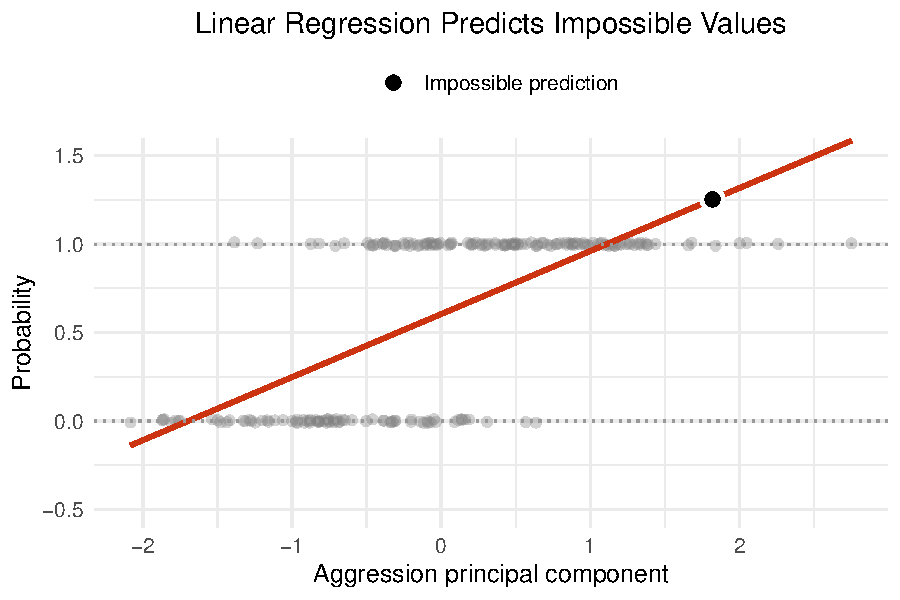
\includegraphics[width=0.8\linewidth,height=\textheight,keepaspectratio]{Beyond!!!_files/figure-pdf/unnamed-chunk-2-1.pdf}
\end{center}

\begin{enumerate}
\def\labelenumi{\arabic{enumi}.}
\setcounter{enumi}{1}
\tightlist
\item
  \ul{Uneven ``noise'' (Heteroskedasticity)}
\end{enumerate}

Linear regression assumes that prediction errors are both normally
distributed and have constant variance across all predicted values.
Binary outcomes violate both assumptions.

\textbf{The problem:} With a 0/1 outcome, the prediction error depends
entirely on the predicted probability:

\begin{itemize}
\tightlist
\item
  If the true label is \textbf{0} and we predict probability \texttt{p},
  the error is \texttt{-p}
\item
  If the true label is \textbf{1} and we predict probability \texttt{p},
  the error is \texttt{1-p}
\end{itemize}

\textbf{Why this matters:} The magnitude of possible errors varies
dramatically with our predicted probability:

\begin{itemize}
\tightlist
\item
  When \texttt{p\ ≈\ 0.50}, errors can be as large as ±0.50
\item
  When \texttt{p\ ≈\ 0.95}, errors shrink to just ±0.05
\end{itemize}

This uneven reliability violates linear regression's core assumption of
constant error variance, making the model's confidence intervals and
p-values unreliable across different probability ranges.

\textbf{The consequence:} Since ordinary linear regression assumes
constant error variance, its confidence intervals and p-values become
unreliable when applied to binary data. The model ``thinks'' it's more
precise than it actually is in some regions and less precise in others.

\begin{center}
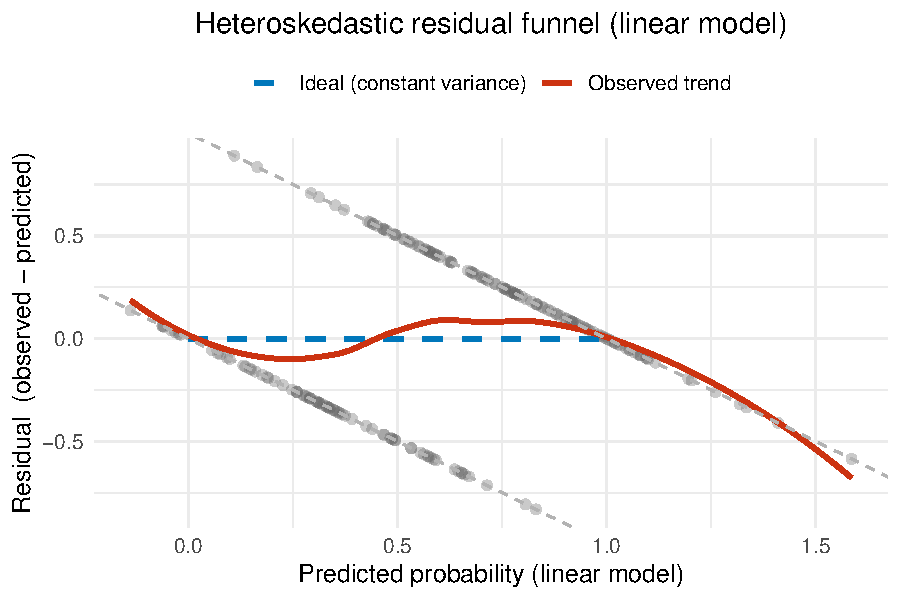
\includegraphics[width=0.8\linewidth,height=\textheight,keepaspectratio]{Beyond!!!_files/figure-pdf/unnamed-chunk-3-1.pdf}
\end{center}

These fundamental problems mean we need a different approach---one that
respects probability boundaries and properly handles binary data's
quirks. This is where logistic regression shines.

\subsubsection{How Logistic Regression Fixes
It}\label{how-logistic-regression-fixes-it}

Logistic regression places the linear combination inside a curve that
automatically constrains predictions between {[}0, 1{]}:

\[p(\text{spam}) = \frac{1}{1 + e^{-(\beta_0 + \beta_1 \times \text{aggression} + \beta_2 \times \text{word count} + ...)}}\]

Inside the parentheses is still a plain-vanilla linear combination; the
\emph{logistic} curve just keeps the final number honest.

\textbf{But here's the rub:} While this S-shaped curve solves our
boundary problem, it creates a new headache. The relationship between
our predictors and the probability is now curved---a one-unit increase
in ``aggression'' might bump spam probability from 10\% to 15\% in one
region, but only from 90\% to 91\% in another. This makes coefficients
nearly impossible to interpret and statistical inference a nightmare.

\begin{center}
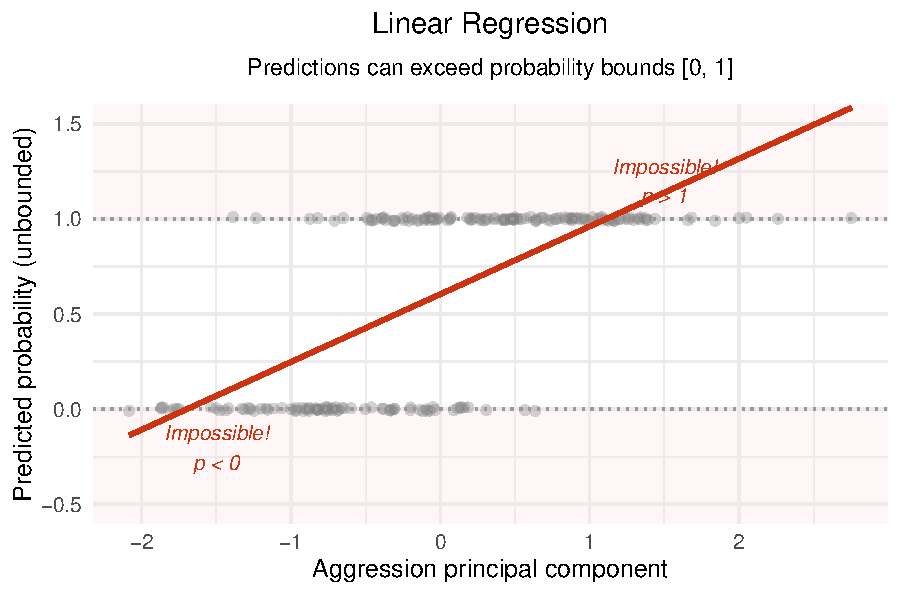
\includegraphics[width=0.8\linewidth,height=\textheight,keepaspectratio]{Beyond!!!_files/figure-pdf/unnamed-chunk-4-1.pdf}
\end{center}

\begin{center}
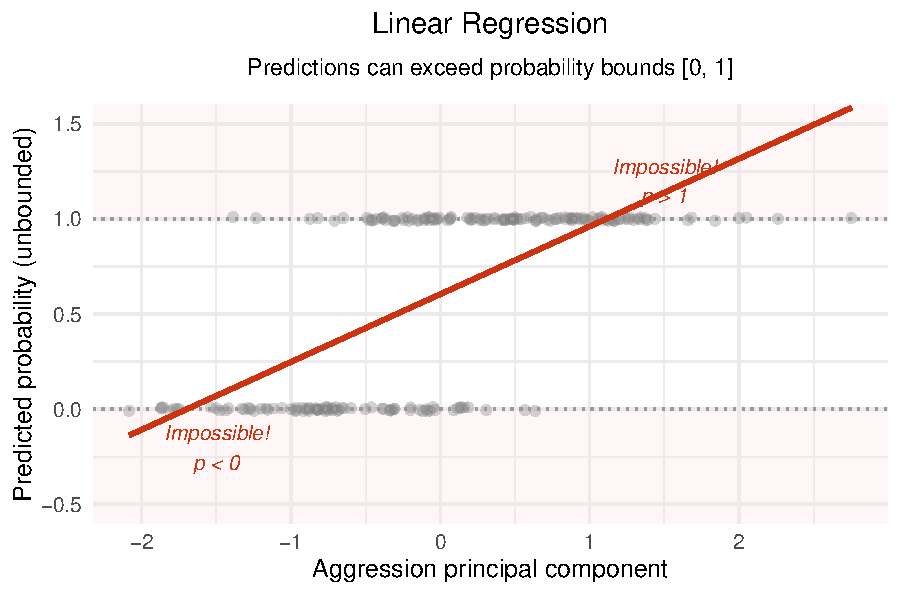
\includegraphics[width=0.8\linewidth,height=\textheight,keepaspectratio]{Beyond!!!_files/figure-pdf/unnamed-chunk-4-2.pdf}
\end{center}

\begin{center}
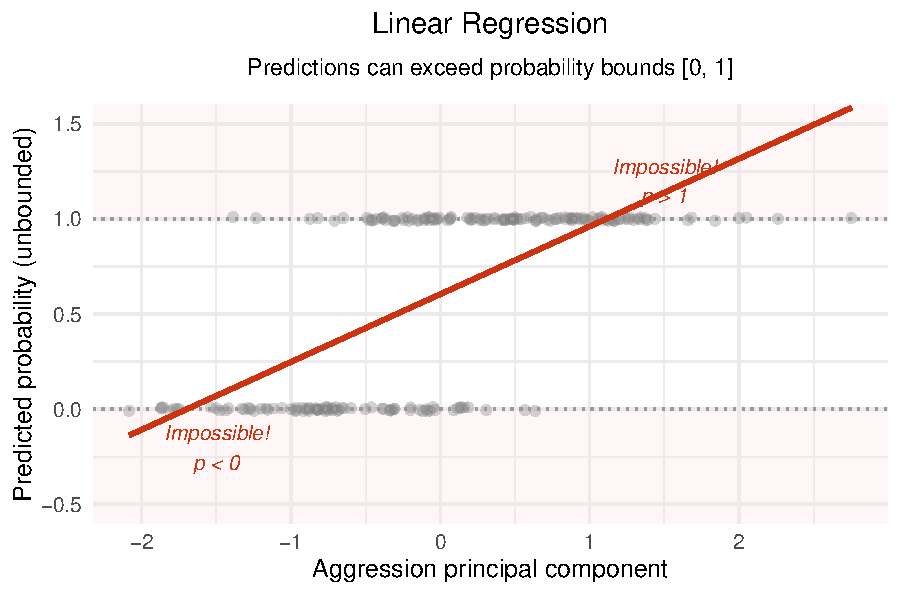
\includegraphics[width=0.8\linewidth,height=\textheight,keepaspectratio]{Beyond!!!_files/figure-pdf/unnamed-chunk-4-3.pdf}
\end{center}

\begin{center}
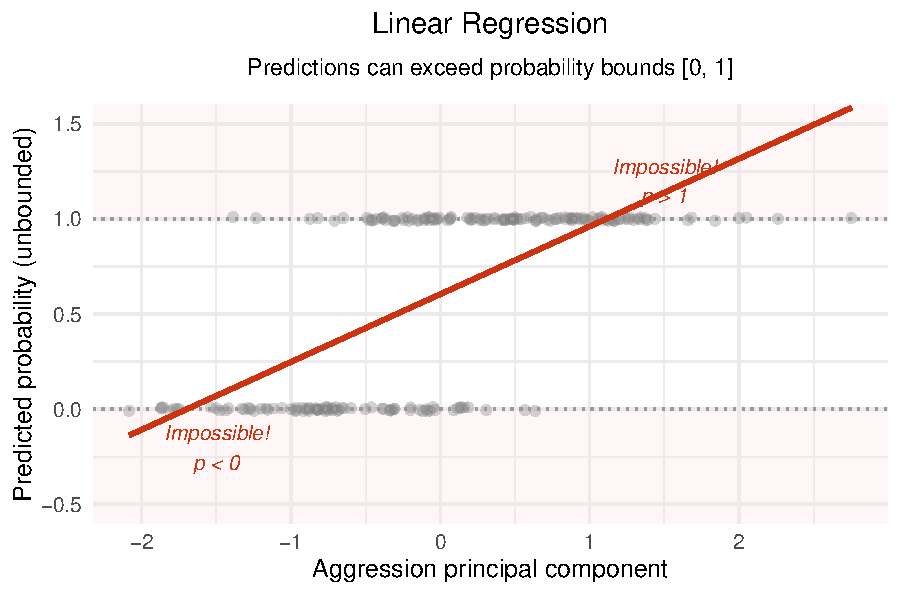
\includegraphics[width=0.8\linewidth,height=\textheight,keepaspectratio]{Beyond!!!_files/figure-pdf/unnamed-chunk-4-4.pdf}
\end{center}

\begin{center}
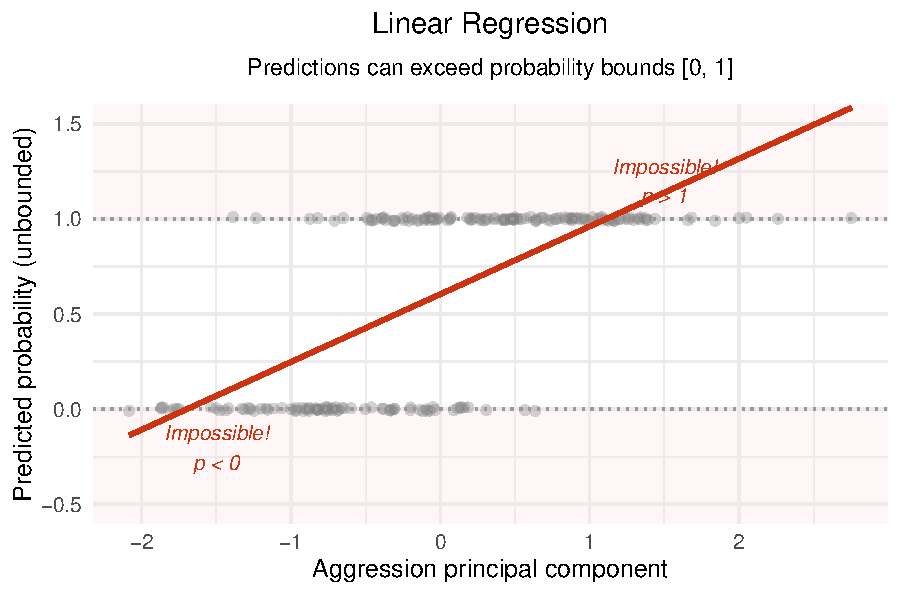
\includegraphics[width=0.8\linewidth,height=\textheight,keepaspectratio]{Beyond!!!_files/figure-pdf/unnamed-chunk-4-5.pdf}
\end{center}

\begin{center}
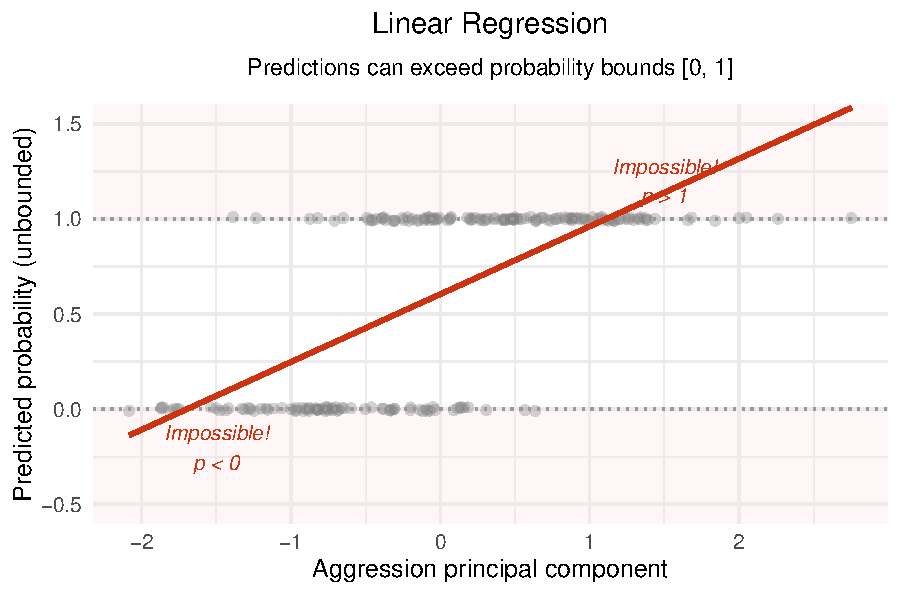
\includegraphics[width=0.8\linewidth,height=\textheight,keepaspectratio]{Beyond!!!_files/figure-pdf/unnamed-chunk-4-6.pdf}
\end{center}

\begin{center}
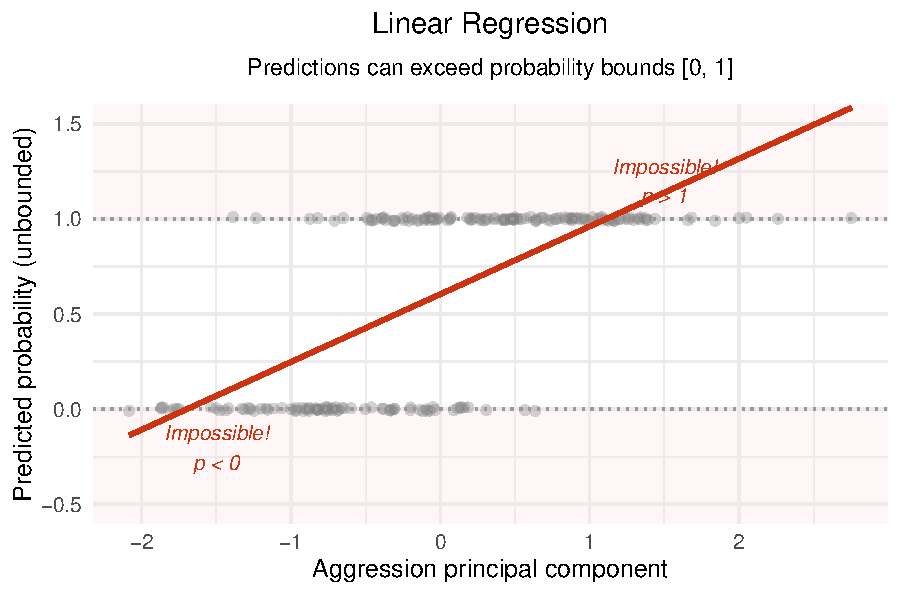
\includegraphics[width=0.8\linewidth,height=\textheight,keepaspectratio]{Beyond!!!_files/figure-pdf/unnamed-chunk-4-7.pdf}
\end{center}

\begin{center}
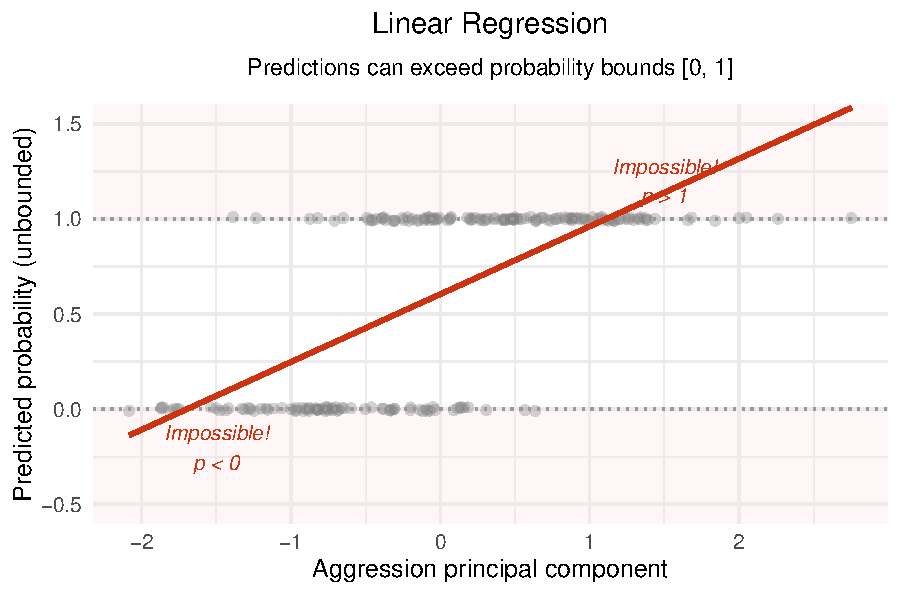
\includegraphics[width=0.8\linewidth,height=\textheight,keepaspectratio]{Beyond!!!_files/figure-pdf/unnamed-chunk-4-8.pdf}
\end{center}

\begin{center}
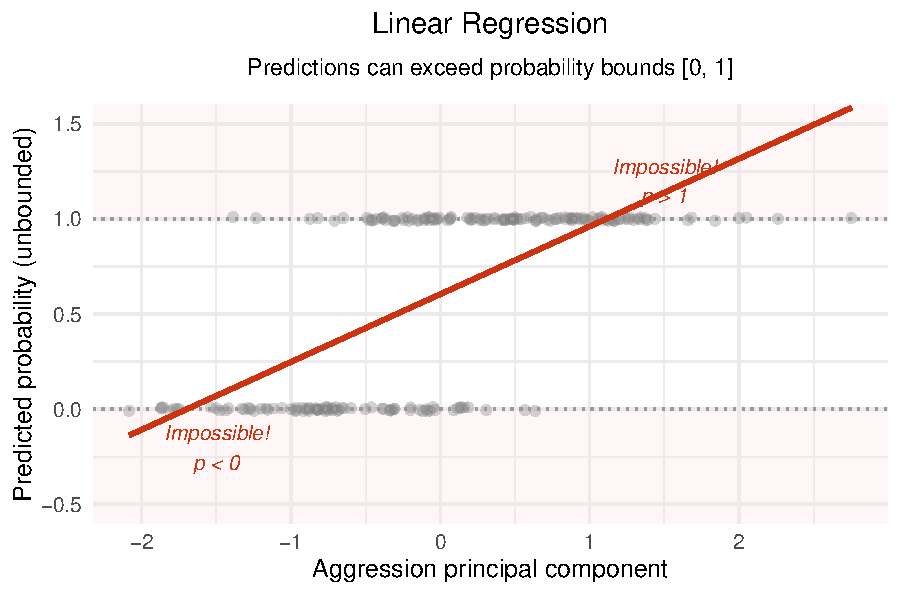
\includegraphics[width=0.8\linewidth,height=\textheight,keepaspectratio]{Beyond!!!_files/figure-pdf/unnamed-chunk-4-9.pdf}
\end{center}

\begin{center}
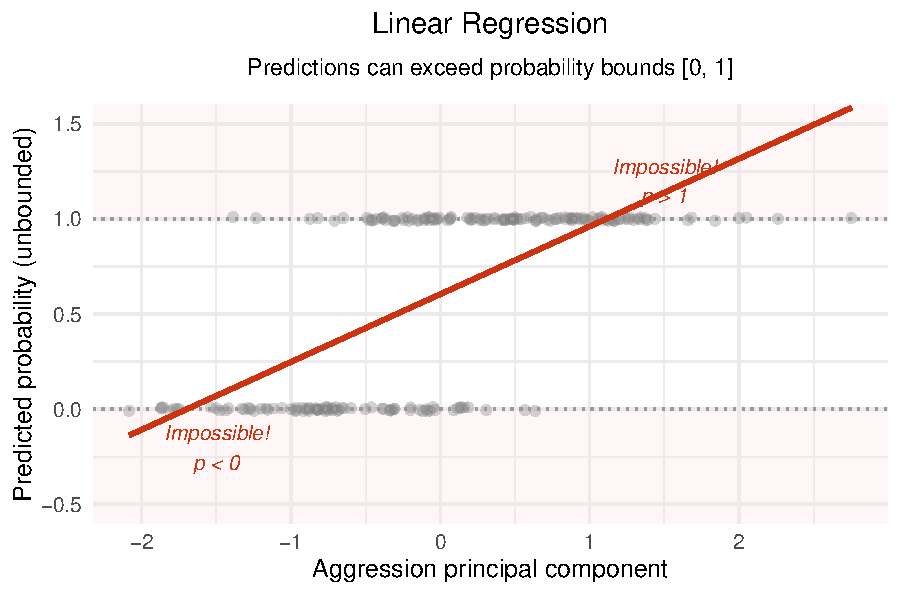
\includegraphics[width=0.8\linewidth,height=\textheight,keepaspectratio]{Beyond!!!_files/figure-pdf/unnamed-chunk-4-10.pdf}
\end{center}

\begin{center}
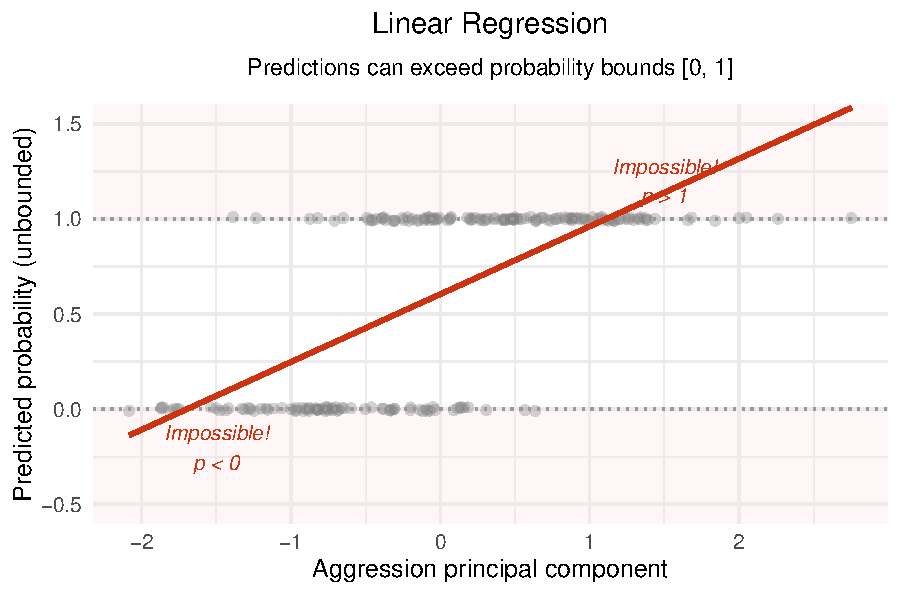
\includegraphics[width=0.8\linewidth,height=\textheight,keepaspectratio]{Beyond!!!_files/figure-pdf/unnamed-chunk-4-11.pdf}
\end{center}

\begin{center}
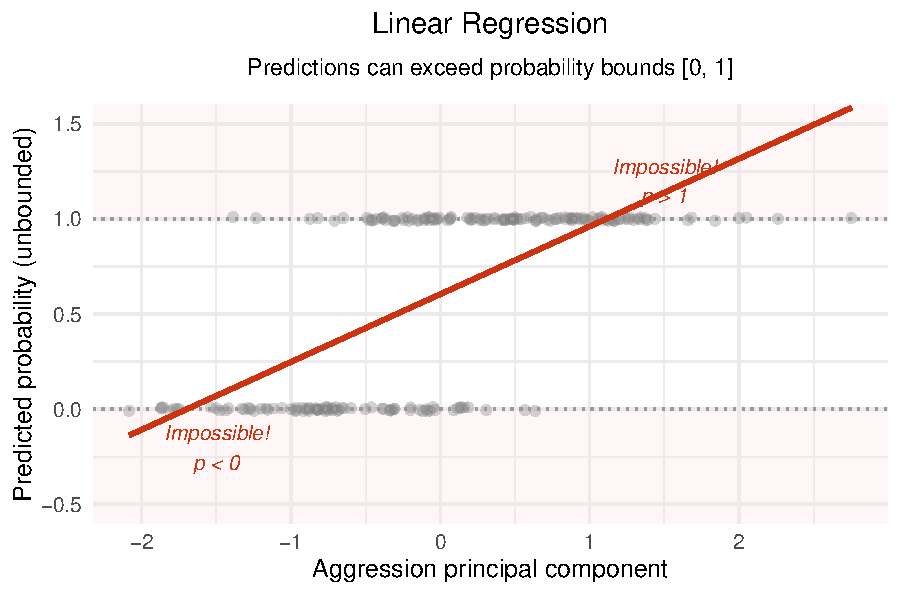
\includegraphics[width=0.8\linewidth,height=\textheight,keepaspectratio]{Beyond!!!_files/figure-pdf/unnamed-chunk-4-12.pdf}
\end{center}

\begin{center}
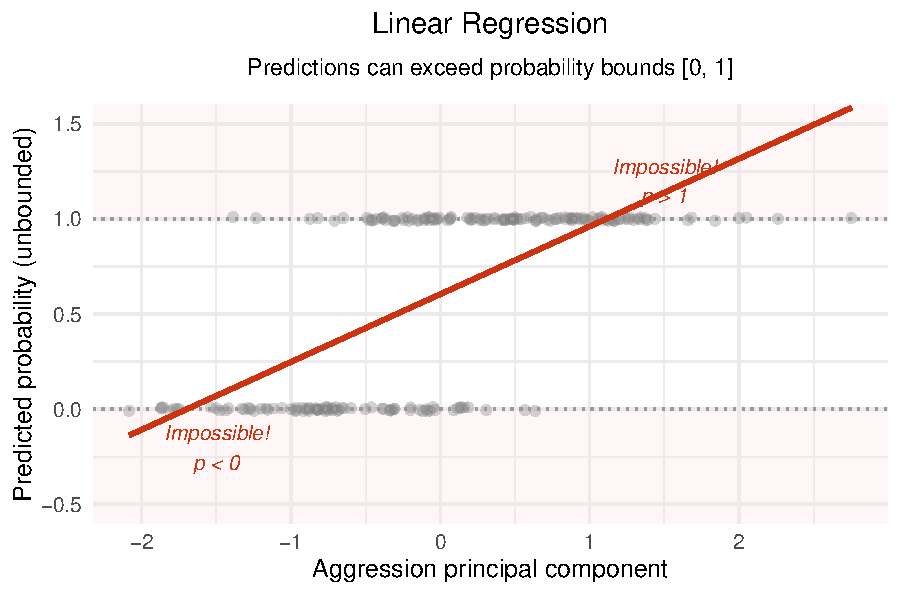
\includegraphics[width=0.8\linewidth,height=\textheight,keepaspectratio]{Beyond!!!_files/figure-pdf/unnamed-chunk-4-13.pdf}
\end{center}

\begin{center}
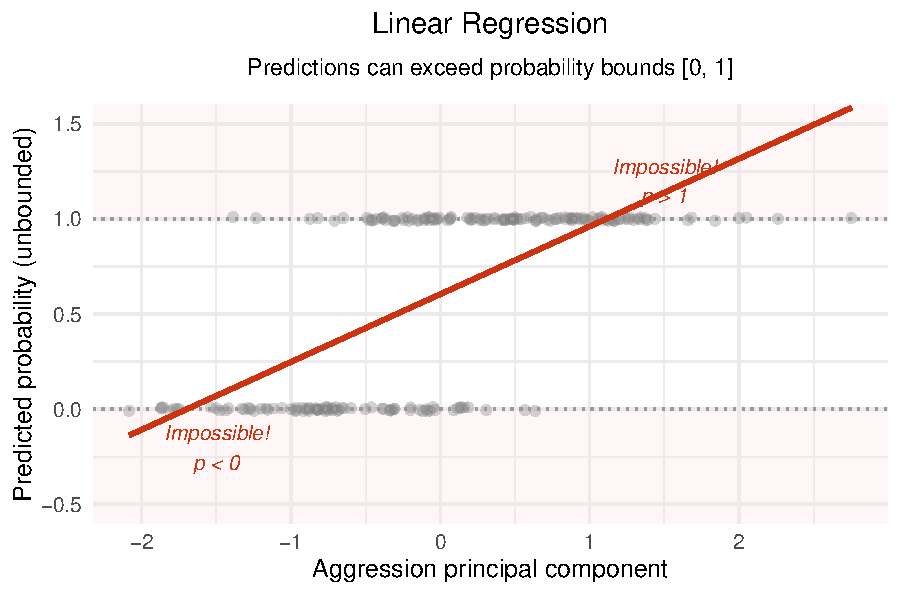
\includegraphics[width=0.8\linewidth,height=\textheight,keepaspectratio]{Beyond!!!_files/figure-pdf/unnamed-chunk-4-14.pdf}
\end{center}

\begin{center}
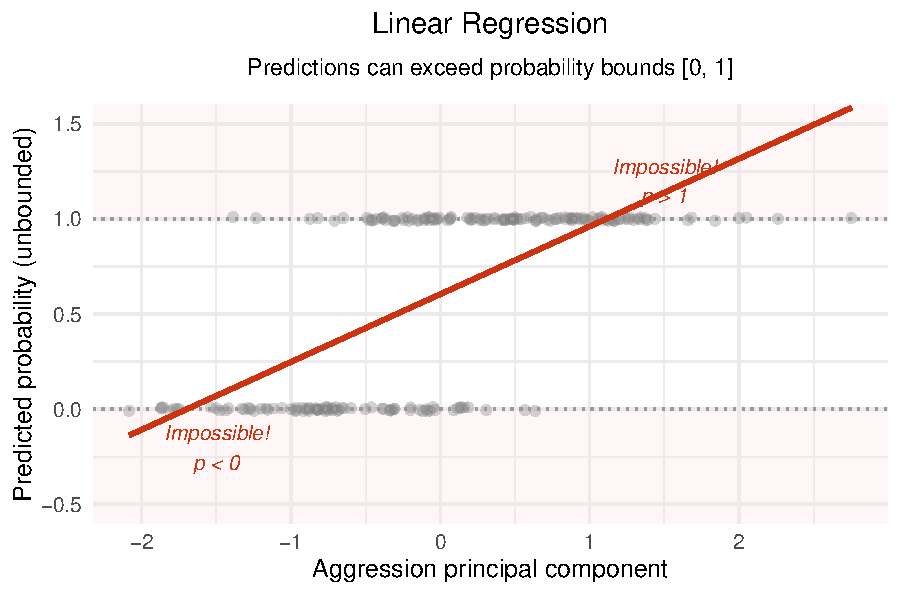
\includegraphics[width=0.8\linewidth,height=\textheight,keepaspectratio]{Beyond!!!_files/figure-pdf/unnamed-chunk-4-15.pdf}
\end{center}

\begin{center}
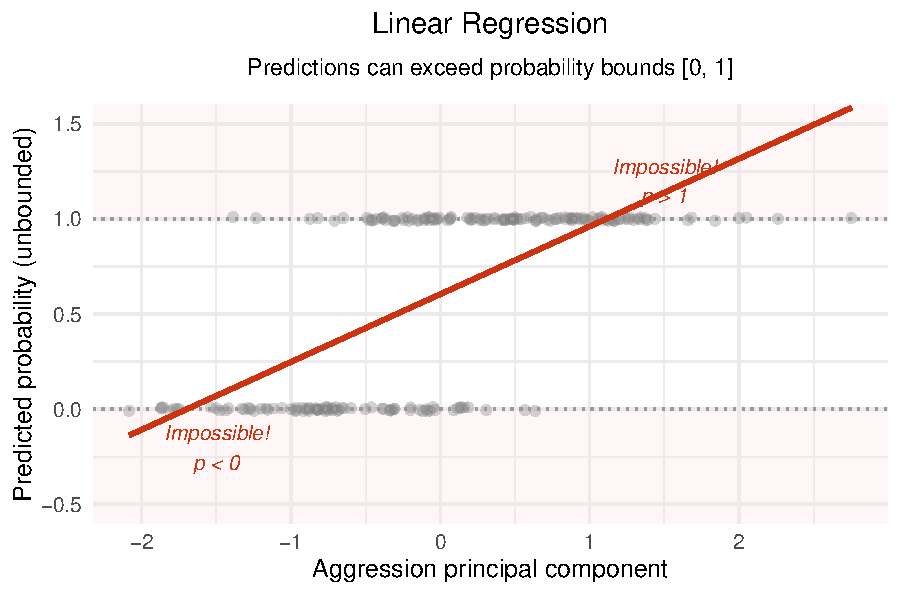
\includegraphics[width=0.8\linewidth,height=\textheight,keepaspectratio]{Beyond!!!_files/figure-pdf/unnamed-chunk-4-16.pdf}
\end{center}

\begin{center}
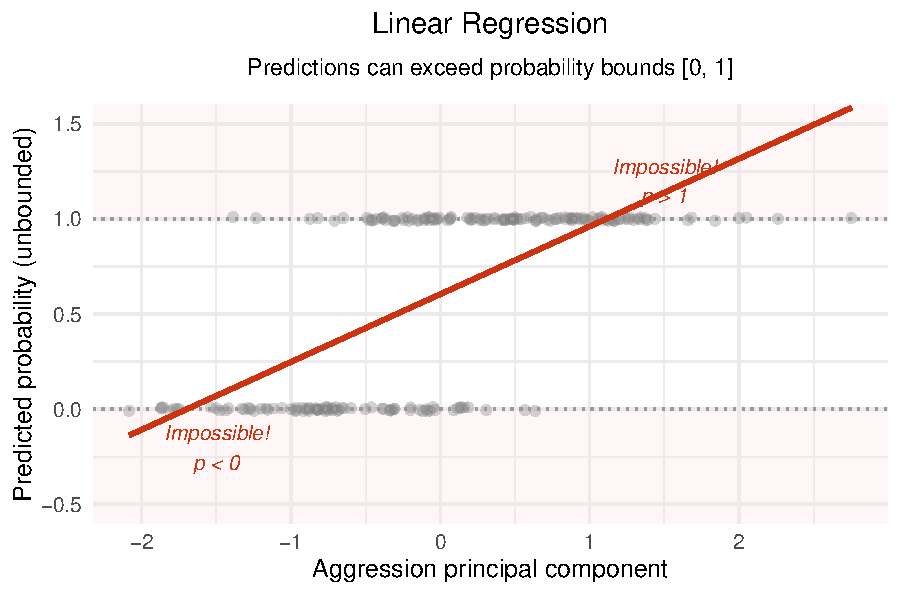
\includegraphics[width=0.8\linewidth,height=\textheight,keepaspectratio]{Beyond!!!_files/figure-pdf/unnamed-chunk-4-17.pdf}
\end{center}

\begin{center}
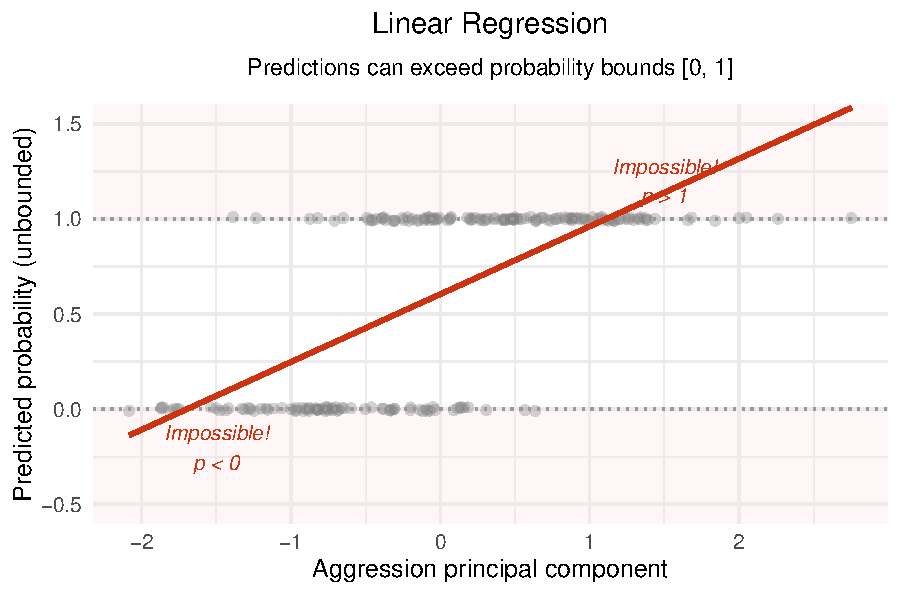
\includegraphics[width=0.8\linewidth,height=\textheight,keepaspectratio]{Beyond!!!_files/figure-pdf/unnamed-chunk-4-18.pdf}
\end{center}

\begin{center}
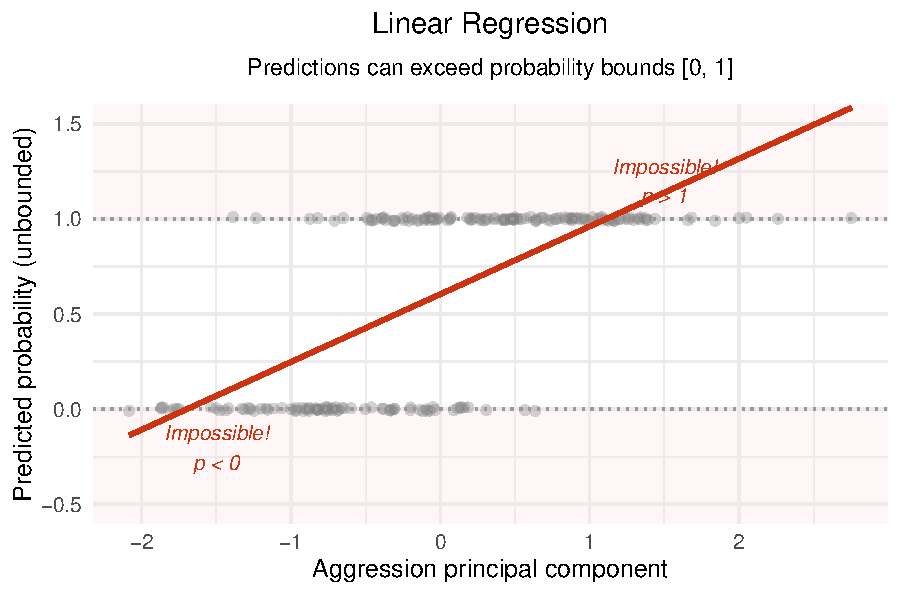
\includegraphics[width=0.8\linewidth,height=\textheight,keepaspectratio]{Beyond!!!_files/figure-pdf/unnamed-chunk-4-19.pdf}
\end{center}

\begin{center}
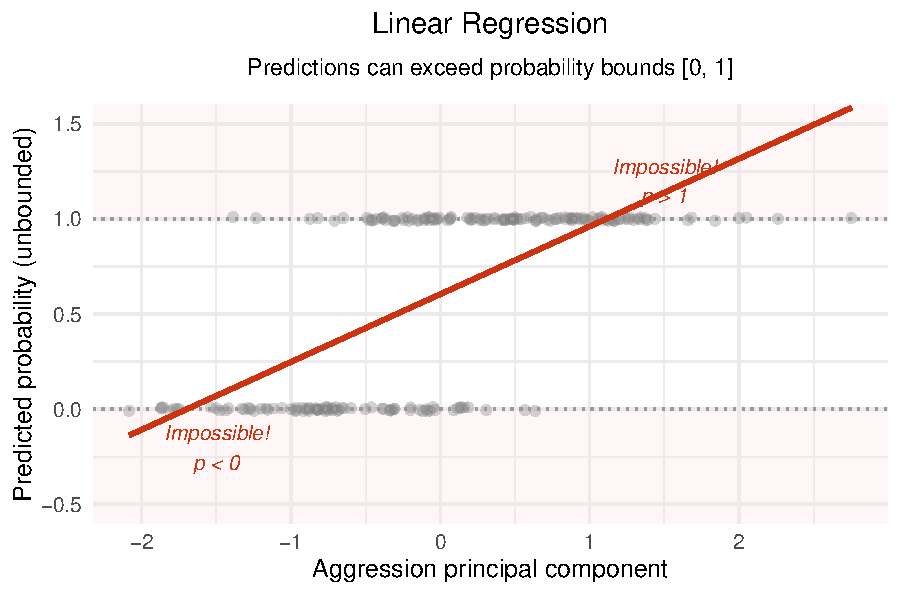
\includegraphics[width=0.8\linewidth,height=\textheight,keepaspectratio]{Beyond!!!_files/figure-pdf/unnamed-chunk-4-20.pdf}
\end{center}

\begin{center}
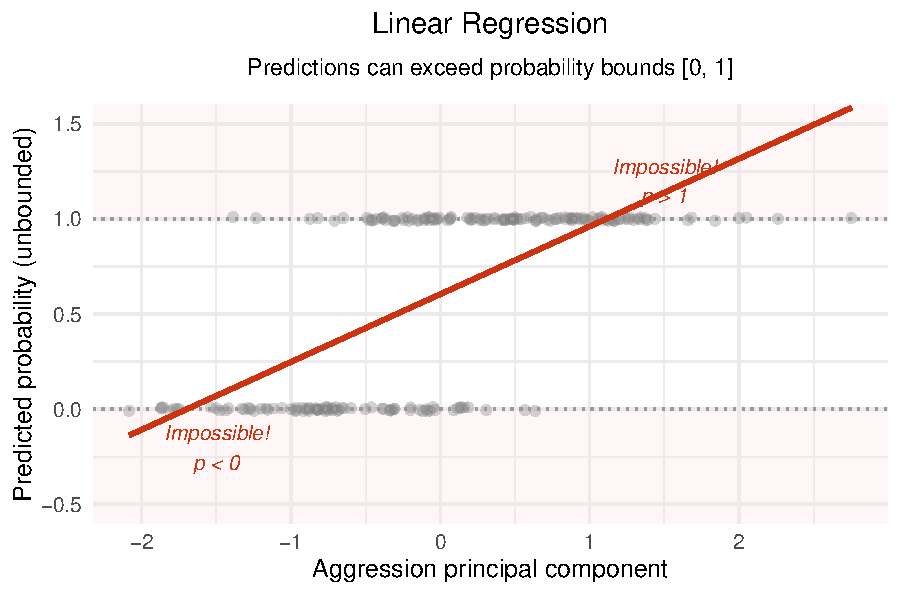
\includegraphics[width=0.8\linewidth,height=\textheight,keepaspectratio]{Beyond!!!_files/figure-pdf/unnamed-chunk-4-21.pdf}
\end{center}

\begin{center}
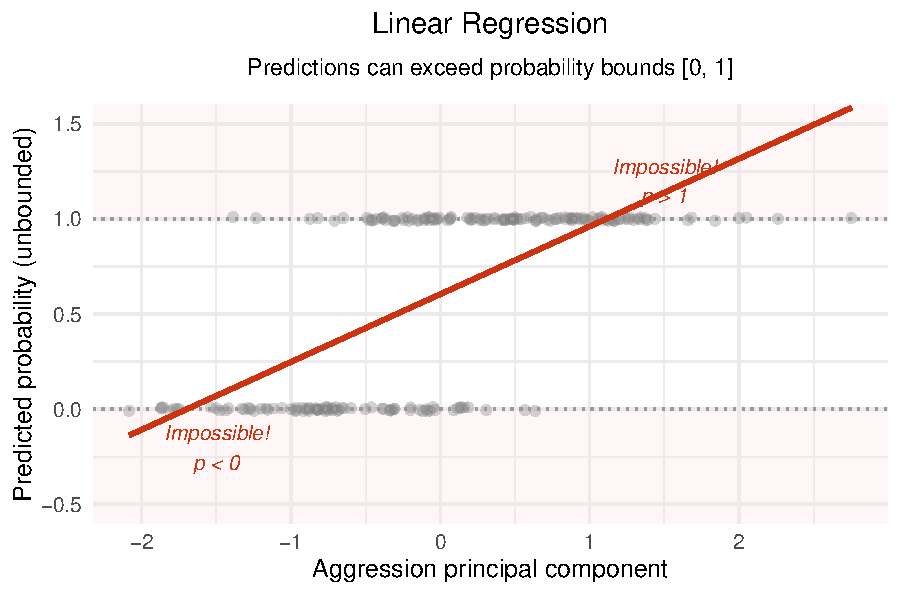
\includegraphics[width=0.8\linewidth,height=\textheight,keepaspectratio]{Beyond!!!_files/figure-pdf/unnamed-chunk-4-22.pdf}
\end{center}

\begin{center}
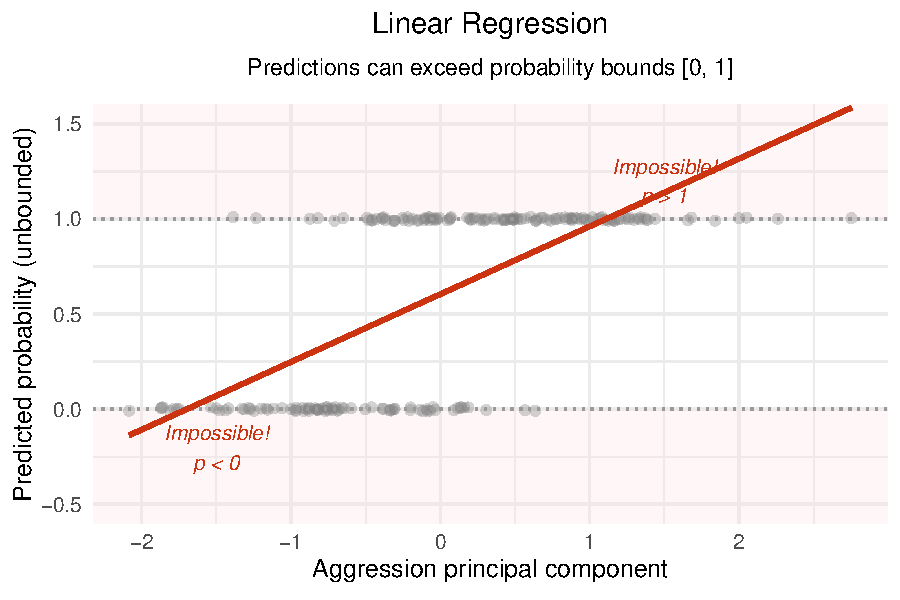
\includegraphics[width=0.8\linewidth,height=\textheight,keepaspectratio]{Beyond!!!_files/figure-pdf/unnamed-chunk-4-23.pdf}
\end{center}

\begin{center}
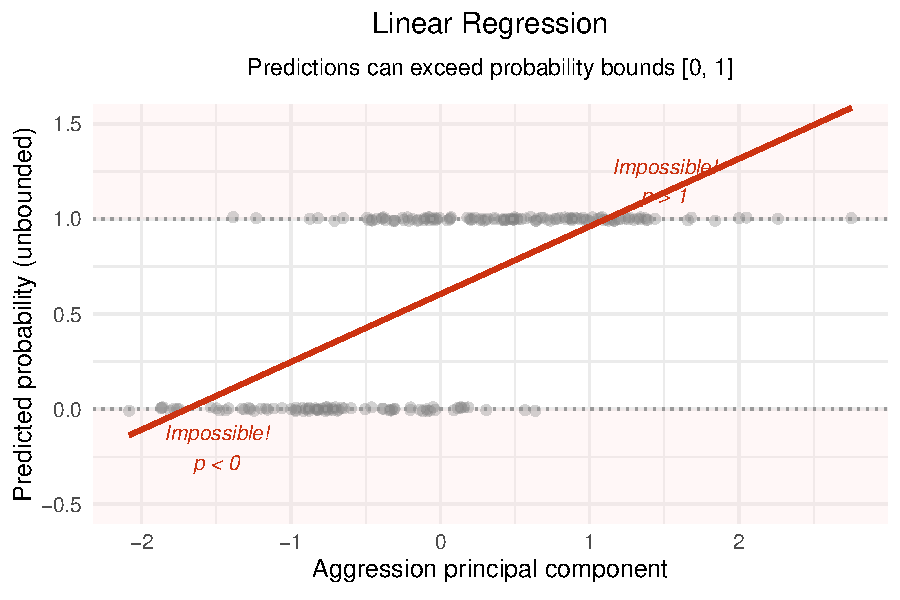
\includegraphics[width=0.8\linewidth,height=\textheight,keepaspectratio]{Beyond!!!_files/figure-pdf/unnamed-chunk-4-24.pdf}
\end{center}

\begin{center}
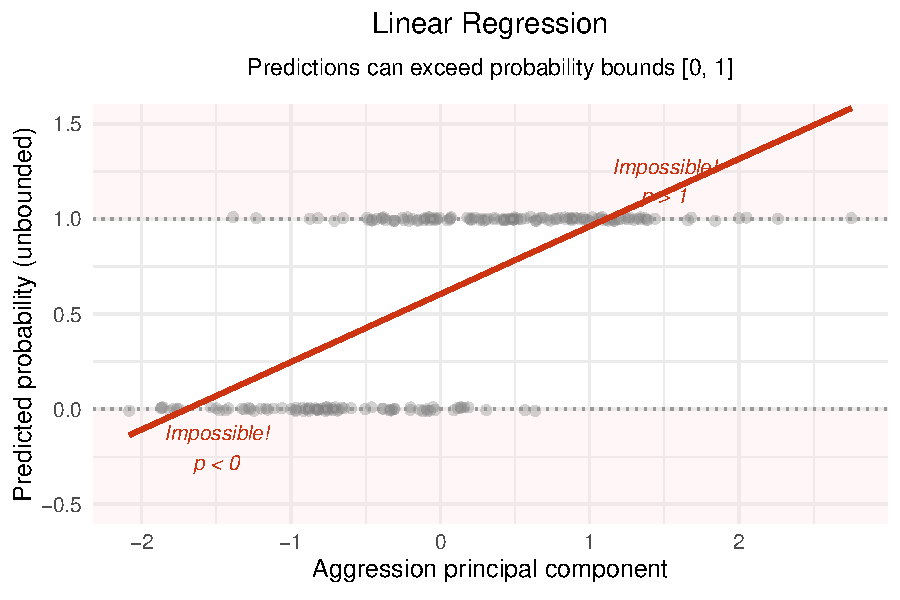
\includegraphics[width=0.8\linewidth,height=\textheight,keepaspectratio]{Beyond!!!_files/figure-pdf/unnamed-chunk-4-25.pdf}
\end{center}

\begin{center}
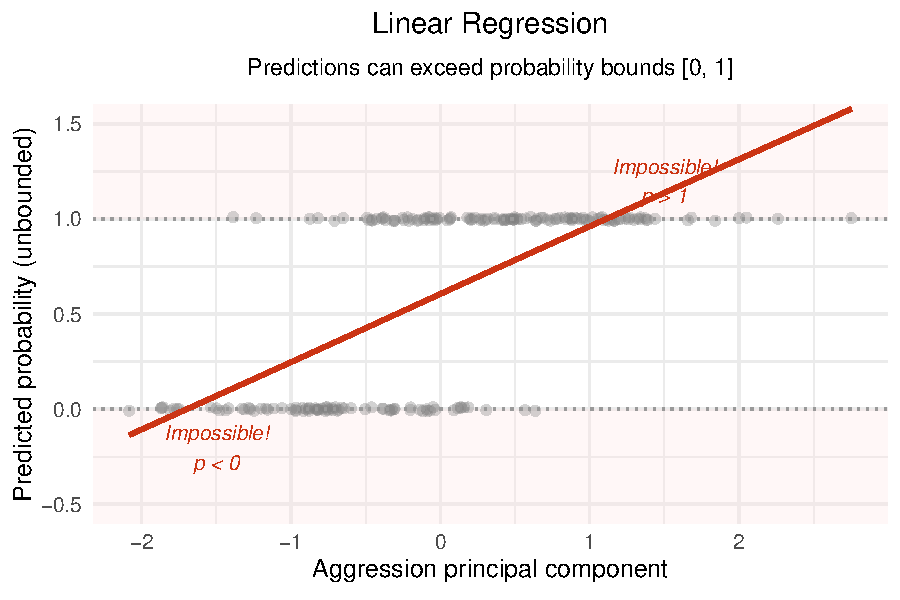
\includegraphics[width=0.8\linewidth,height=\textheight,keepaspectratio]{Beyond!!!_files/figure-pdf/unnamed-chunk-4-26.pdf}
\end{center}

\begin{center}
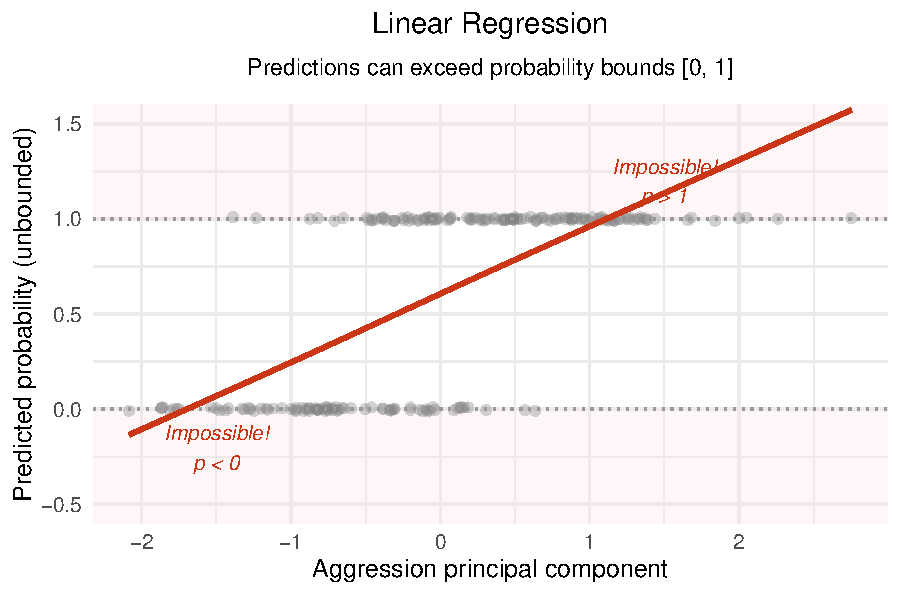
\includegraphics[width=0.8\linewidth,height=\textheight,keepaspectratio]{Beyond!!!_files/figure-pdf/unnamed-chunk-4-27.pdf}
\end{center}

\begin{center}
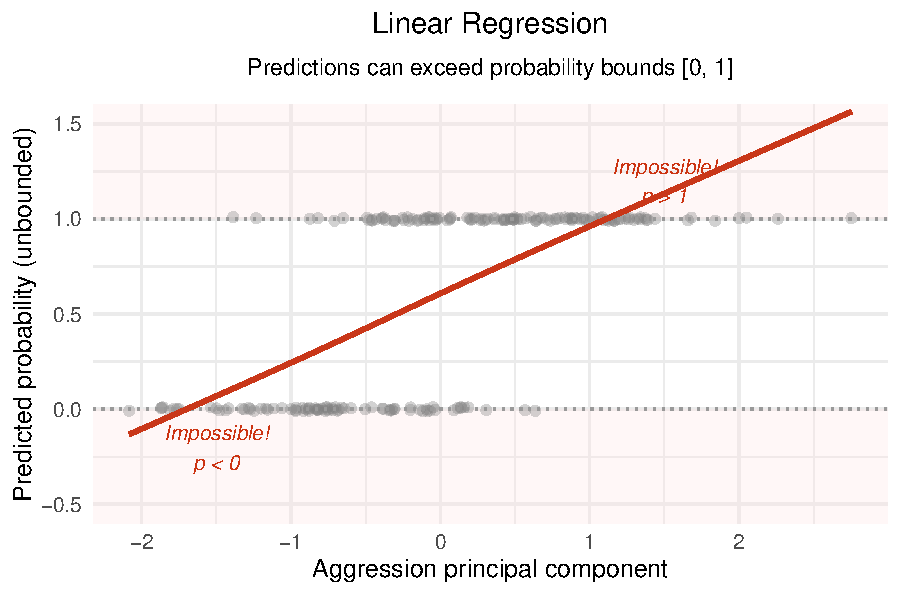
\includegraphics[width=0.8\linewidth,height=\textheight,keepaspectratio]{Beyond!!!_files/figure-pdf/unnamed-chunk-4-28.pdf}
\end{center}

\begin{center}
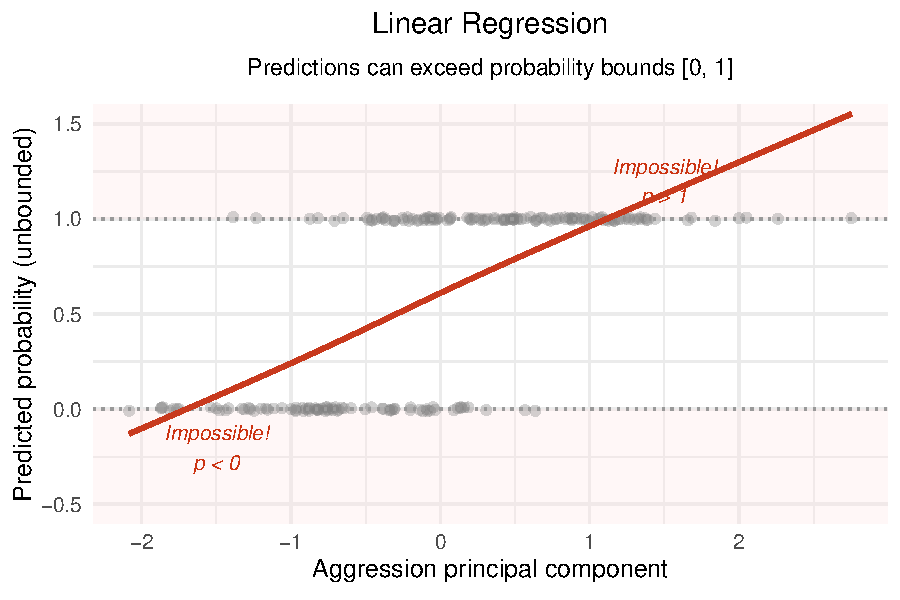
\includegraphics[width=0.8\linewidth,height=\textheight,keepaspectratio]{Beyond!!!_files/figure-pdf/unnamed-chunk-4-29.pdf}
\end{center}

\begin{center}
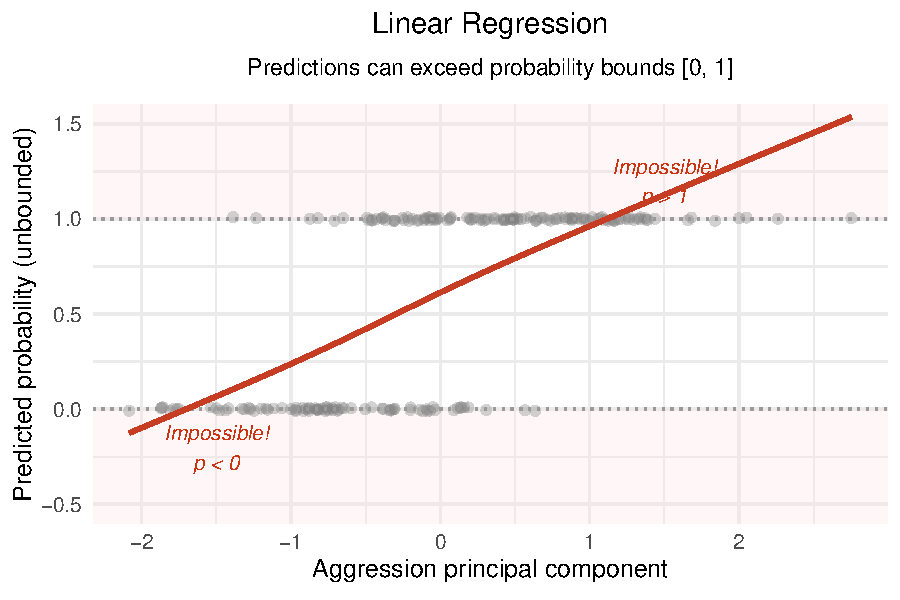
\includegraphics[width=0.8\linewidth,height=\textheight,keepaspectratio]{Beyond!!!_files/figure-pdf/unnamed-chunk-4-30.pdf}
\end{center}

\begin{center}
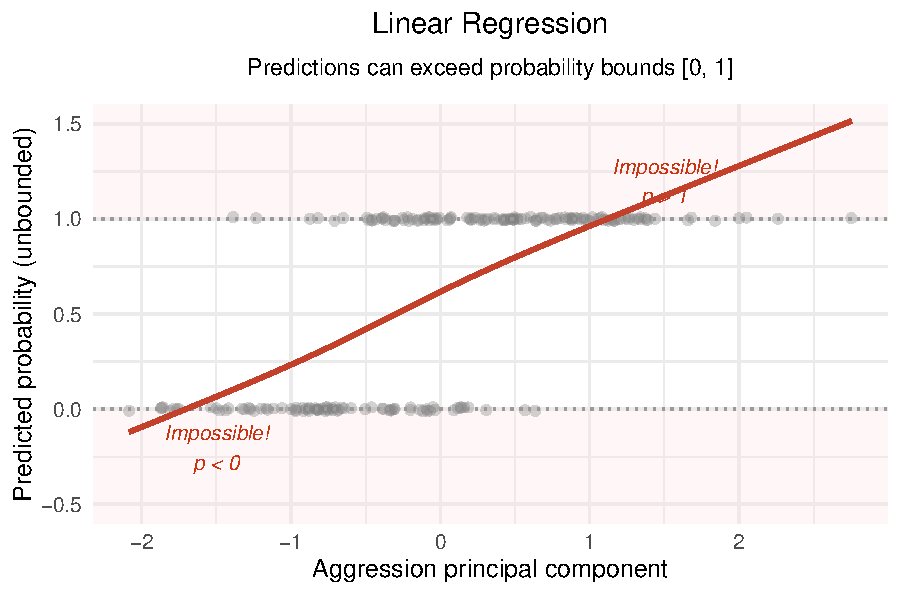
\includegraphics[width=0.8\linewidth,height=\textheight,keepaspectratio]{Beyond!!!_files/figure-pdf/unnamed-chunk-4-31.pdf}
\end{center}

\begin{center}
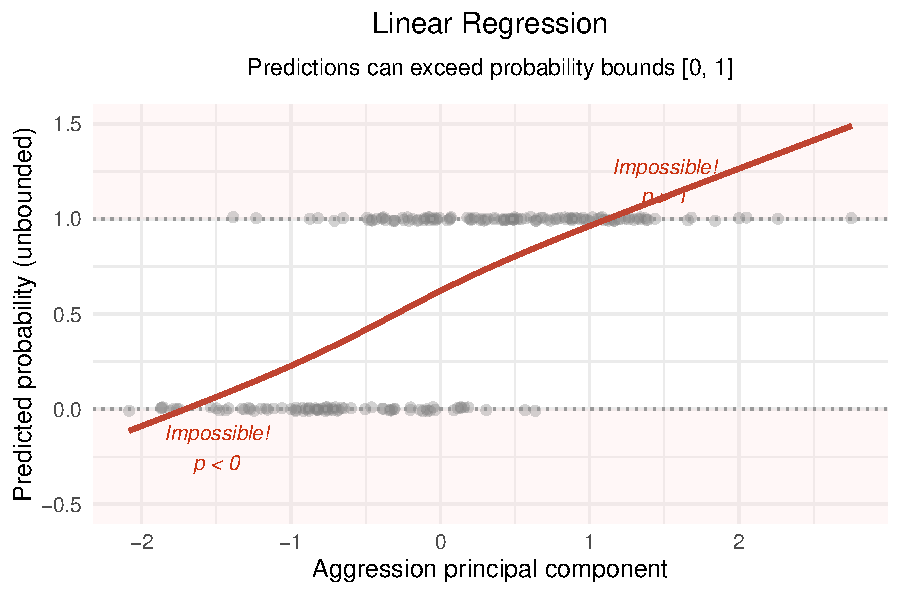
\includegraphics[width=0.8\linewidth,height=\textheight,keepaspectratio]{Beyond!!!_files/figure-pdf/unnamed-chunk-4-32.pdf}
\end{center}

\begin{center}
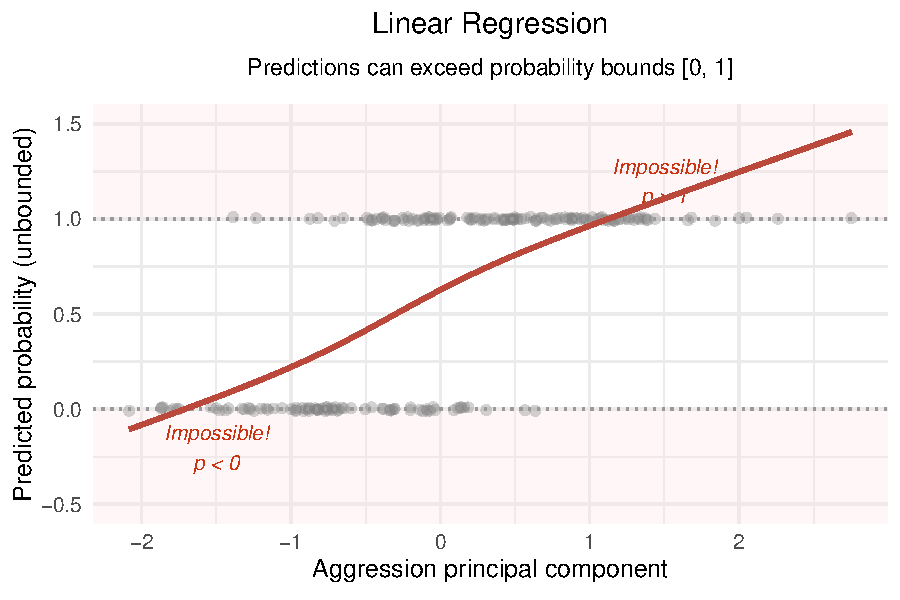
\includegraphics[width=0.8\linewidth,height=\textheight,keepaspectratio]{Beyond!!!_files/figure-pdf/unnamed-chunk-4-33.pdf}
\end{center}

\begin{center}
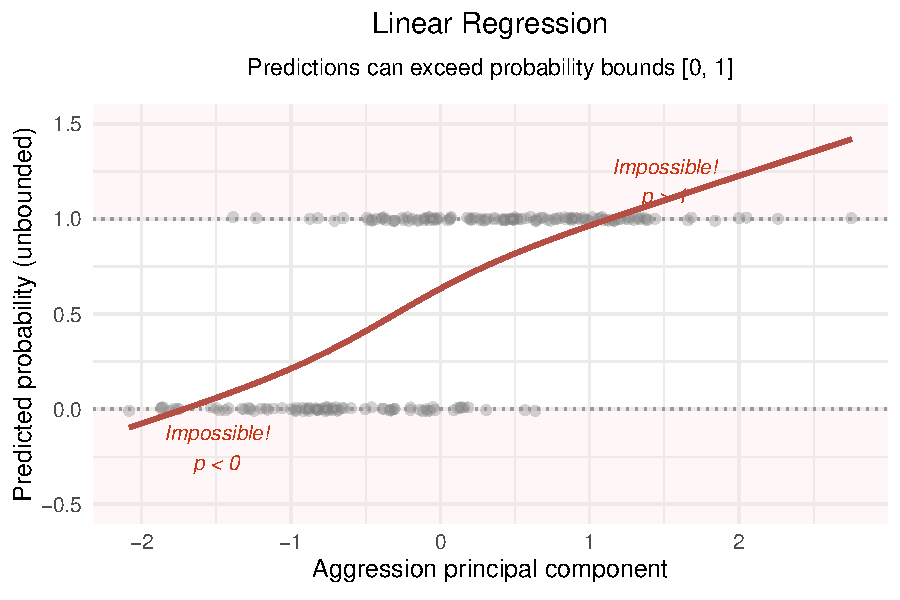
\includegraphics[width=0.8\linewidth,height=\textheight,keepaspectratio]{Beyond!!!_files/figure-pdf/unnamed-chunk-4-34.pdf}
\end{center}

\begin{center}
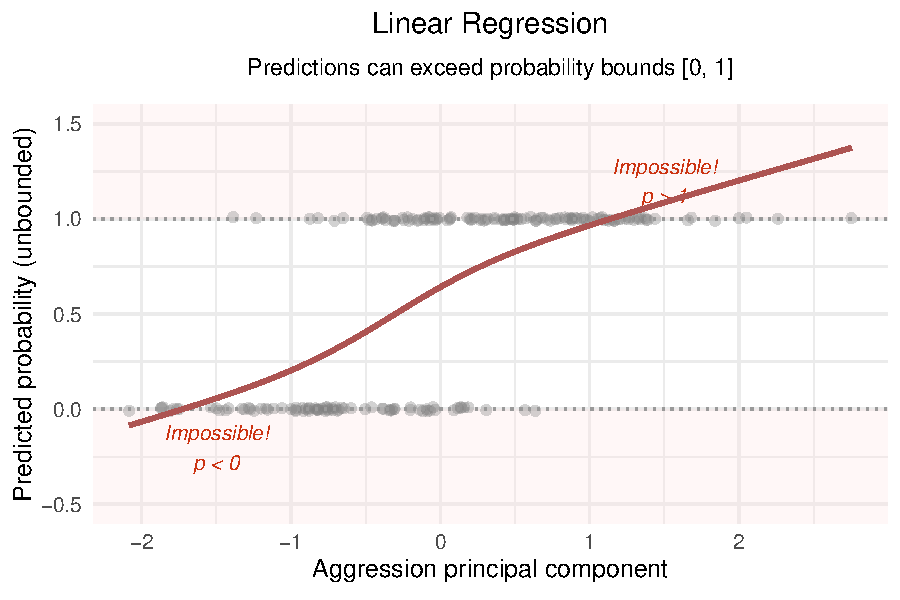
\includegraphics[width=0.8\linewidth,height=\textheight,keepaspectratio]{Beyond!!!_files/figure-pdf/unnamed-chunk-4-35.pdf}
\end{center}

\begin{center}
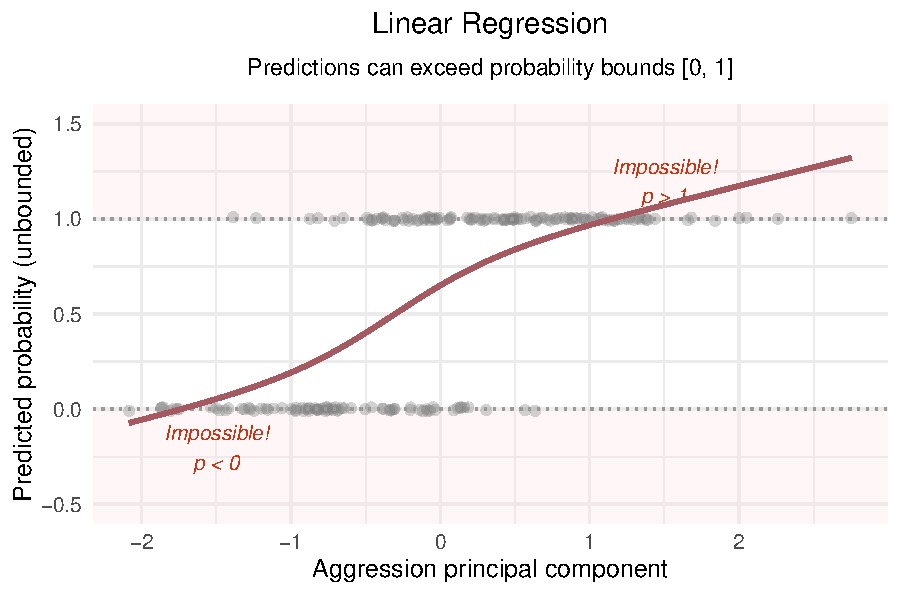
\includegraphics[width=0.8\linewidth,height=\textheight,keepaspectratio]{Beyond!!!_files/figure-pdf/unnamed-chunk-4-36.pdf}
\end{center}

\begin{center}
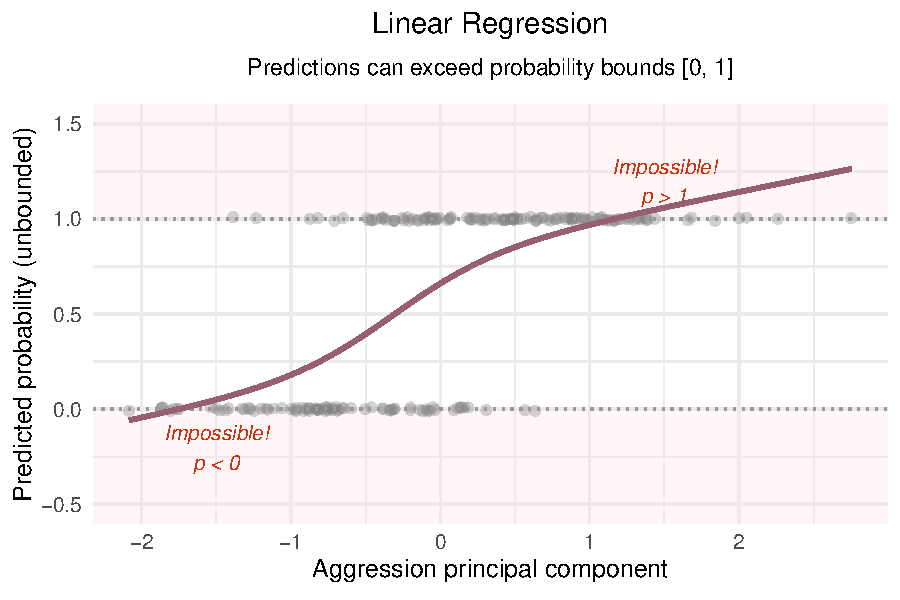
\includegraphics[width=0.8\linewidth,height=\textheight,keepaspectratio]{Beyond!!!_files/figure-pdf/unnamed-chunk-4-37.pdf}
\end{center}

\begin{center}
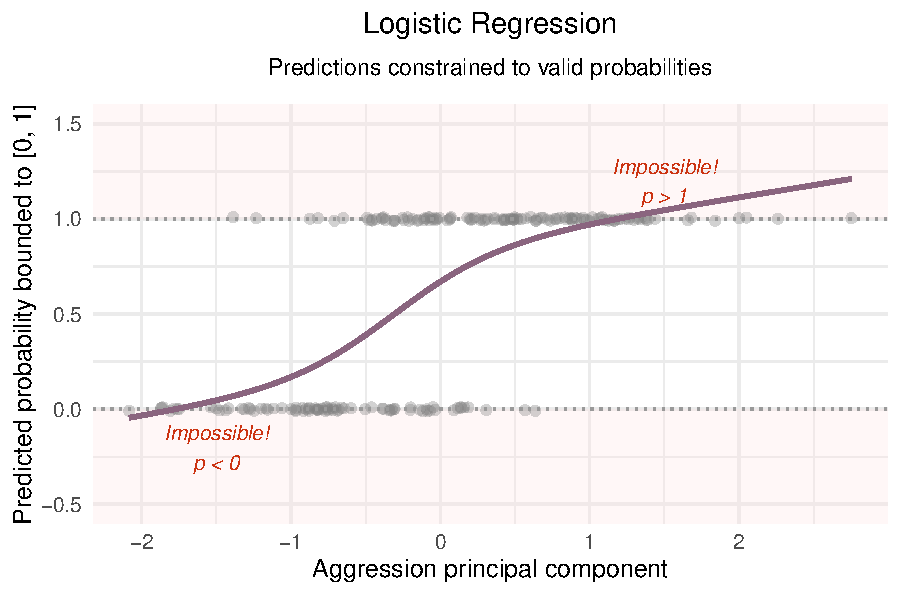
\includegraphics[width=0.8\linewidth,height=\textheight,keepaspectratio]{Beyond!!!_files/figure-pdf/unnamed-chunk-4-38.pdf}
\end{center}

\begin{center}
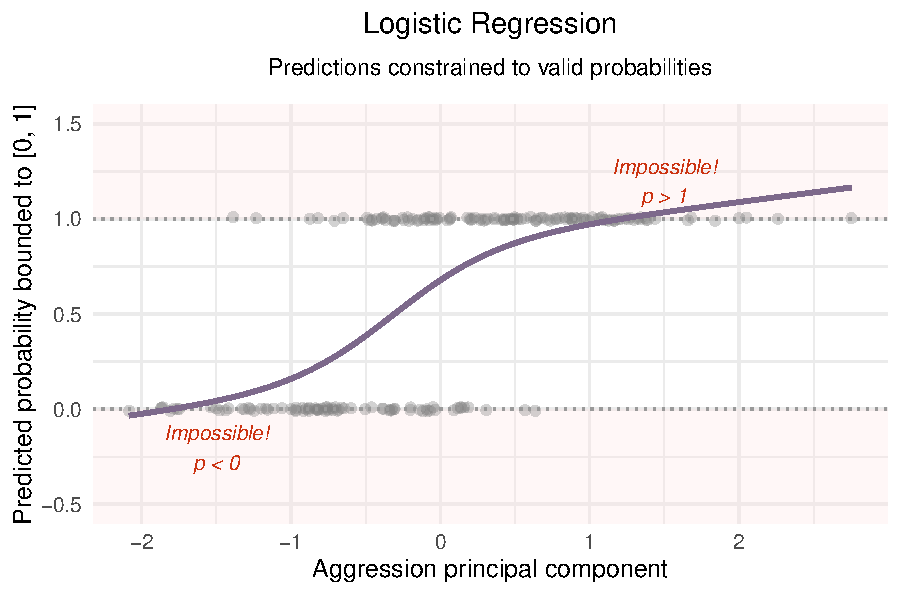
\includegraphics[width=0.8\linewidth,height=\textheight,keepaspectratio]{Beyond!!!_files/figure-pdf/unnamed-chunk-4-39.pdf}
\end{center}

\begin{center}
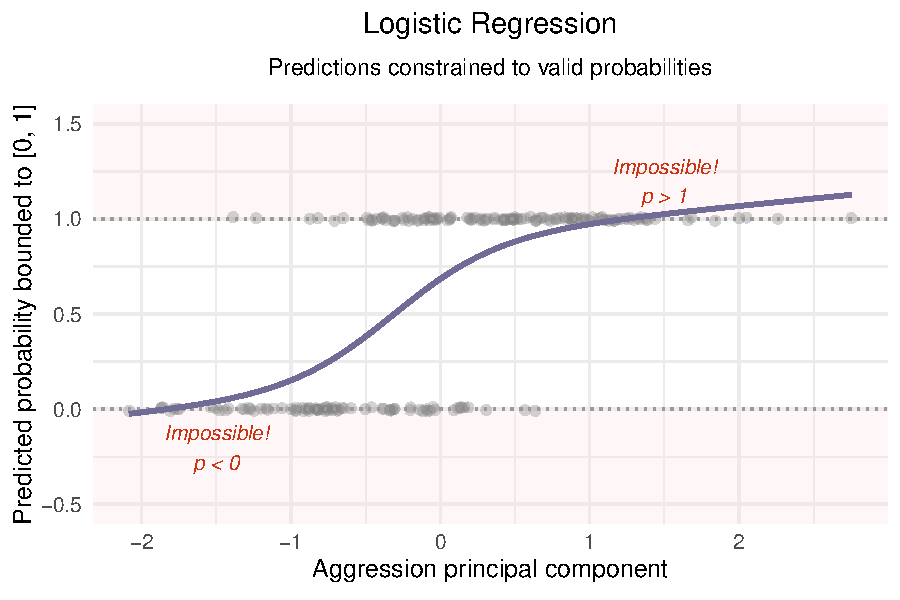
\includegraphics[width=0.8\linewidth,height=\textheight,keepaspectratio]{Beyond!!!_files/figure-pdf/unnamed-chunk-4-40.pdf}
\end{center}

\begin{center}
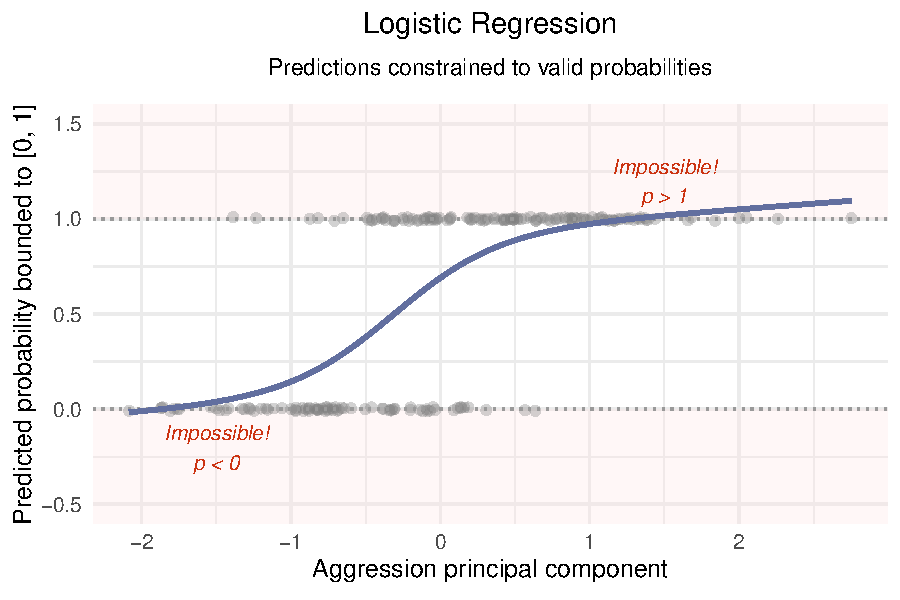
\includegraphics[width=0.8\linewidth,height=\textheight,keepaspectratio]{Beyond!!!_files/figure-pdf/unnamed-chunk-4-41.pdf}
\end{center}

\begin{center}
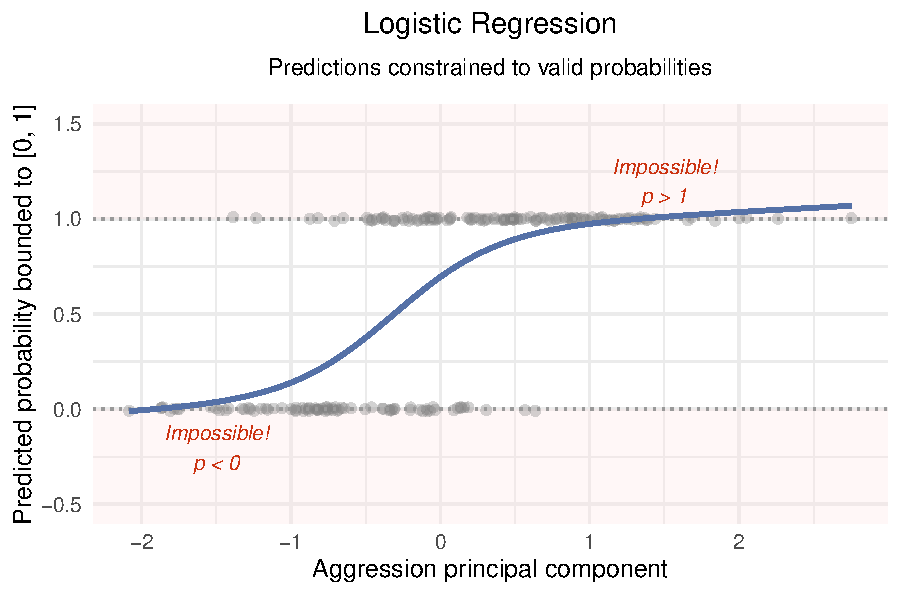
\includegraphics[width=0.8\linewidth,height=\textheight,keepaspectratio]{Beyond!!!_files/figure-pdf/unnamed-chunk-4-42.pdf}
\end{center}

\begin{center}
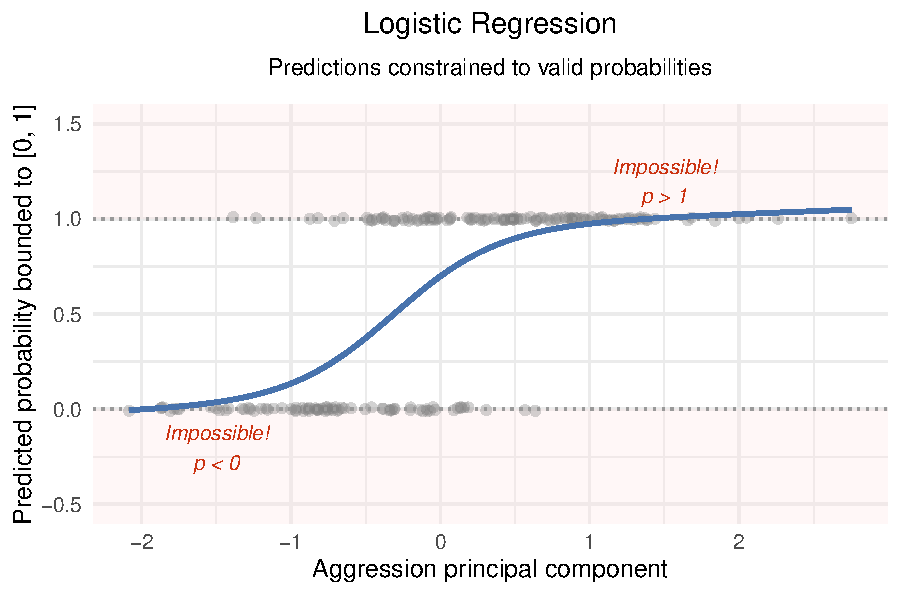
\includegraphics[width=0.8\linewidth,height=\textheight,keepaspectratio]{Beyond!!!_files/figure-pdf/unnamed-chunk-4-43.pdf}
\end{center}

\begin{center}
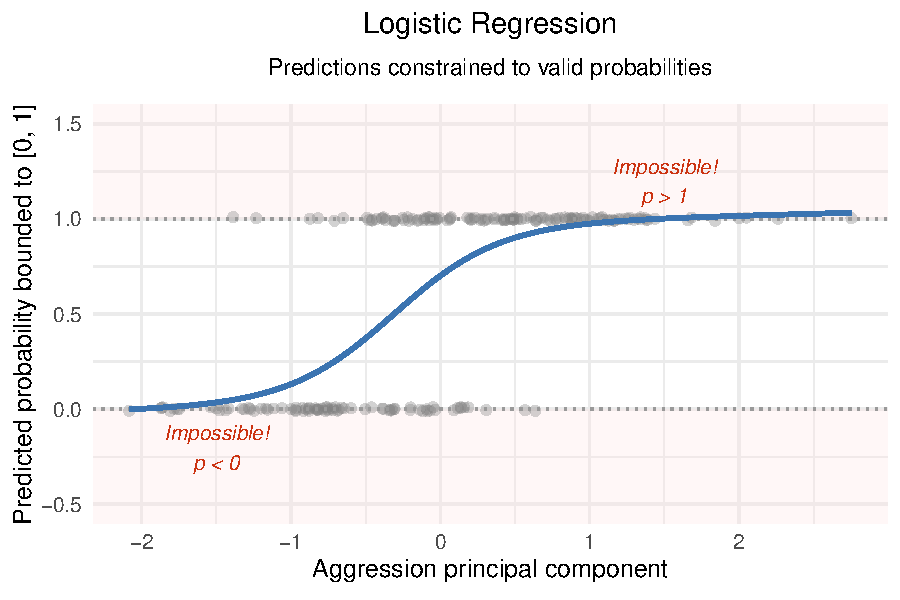
\includegraphics[width=0.8\linewidth,height=\textheight,keepaspectratio]{Beyond!!!_files/figure-pdf/unnamed-chunk-4-44.pdf}
\end{center}

\begin{center}
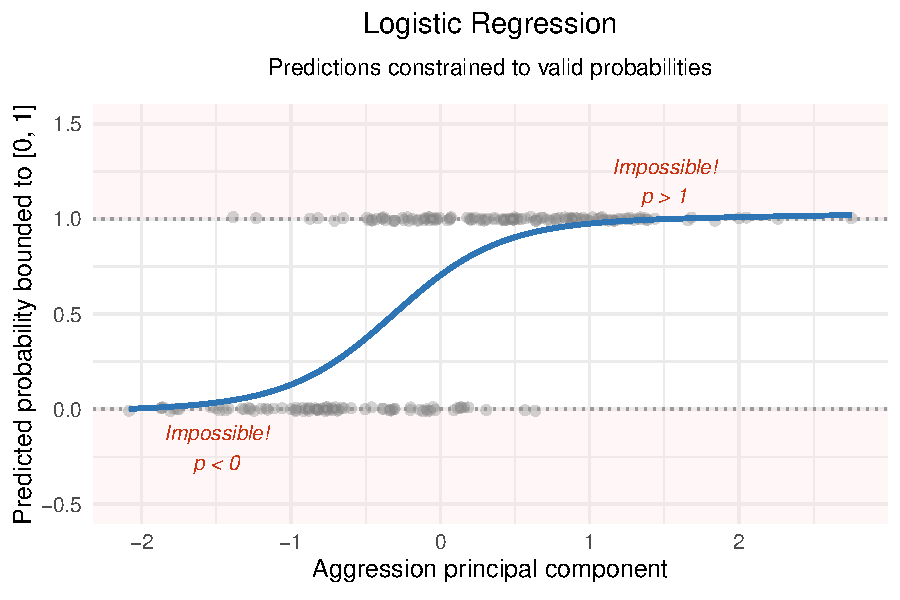
\includegraphics[width=0.8\linewidth,height=\textheight,keepaspectratio]{Beyond!!!_files/figure-pdf/unnamed-chunk-4-45.pdf}
\end{center}

\begin{center}
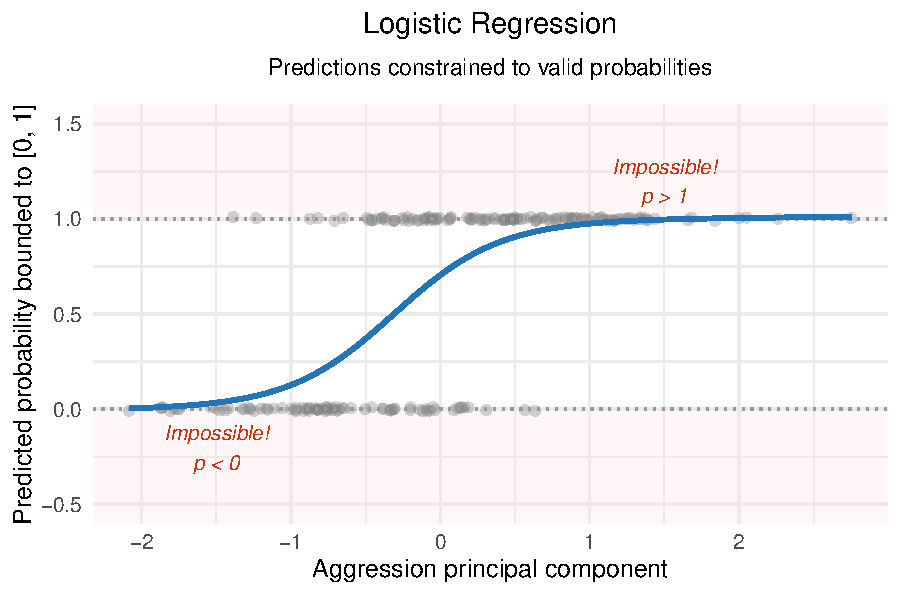
\includegraphics[width=0.8\linewidth,height=\textheight,keepaspectratio]{Beyond!!!_files/figure-pdf/unnamed-chunk-4-46.pdf}
\end{center}

\begin{center}
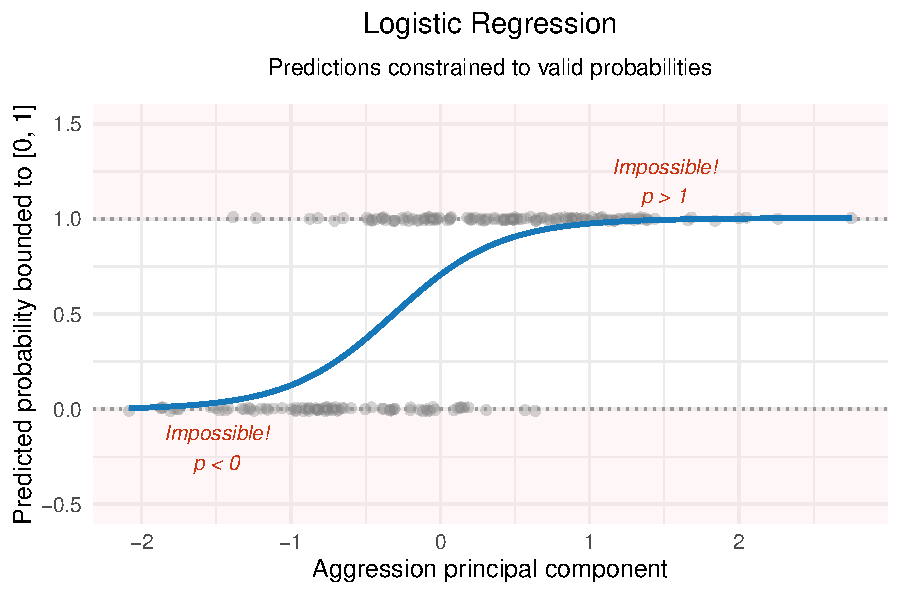
\includegraphics[width=0.8\linewidth,height=\textheight,keepaspectratio]{Beyond!!!_files/figure-pdf/unnamed-chunk-4-47.pdf}
\end{center}

\begin{center}
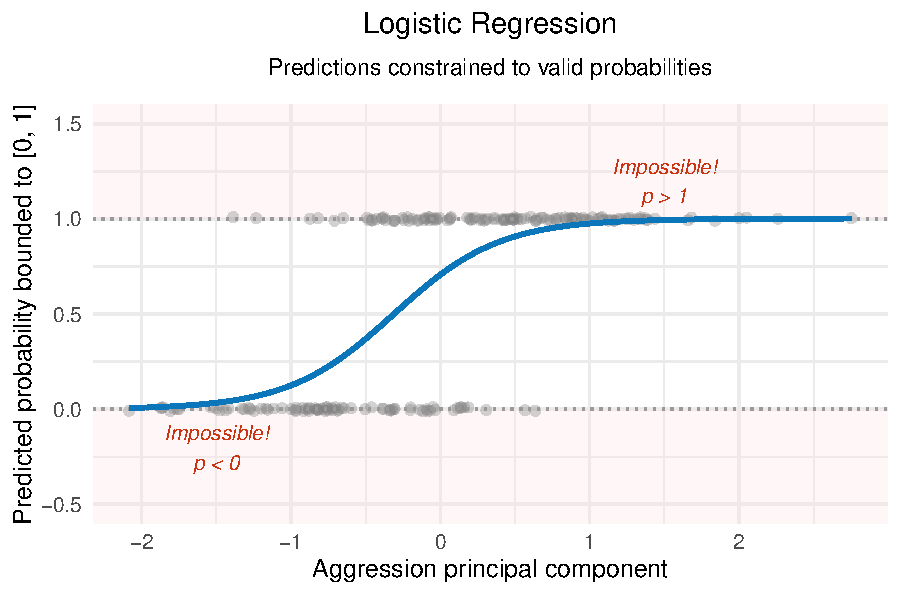
\includegraphics[width=0.8\linewidth,height=\textheight,keepaspectratio]{Beyond!!!_files/figure-pdf/unnamed-chunk-4-48.pdf}
\end{center}

\begin{center}
\includegraphics[width=0.8\linewidth,height=\textheight,keepaspectratio]{Beyond!!!_files/figure-pdf/unnamed-chunk-4-49.pdf}
\end{center}

\begin{center}
\includegraphics[width=0.8\linewidth,height=\textheight,keepaspectratio]{Beyond!!!_files/figure-pdf/unnamed-chunk-4-50.pdf}
\end{center}

\begin{center}
\includegraphics[width=0.8\linewidth,height=\textheight,keepaspectratio]{Beyond!!!_files/figure-pdf/unnamed-chunk-4-51.pdf}
\end{center}

\begin{center}
\includegraphics[width=0.8\linewidth,height=\textheight,keepaspectratio]{Beyond!!!_files/figure-pdf/unnamed-chunk-4-52.pdf}
\end{center}

\begin{center}
\includegraphics[width=0.8\linewidth,height=\textheight,keepaspectratio]{Beyond!!!_files/figure-pdf/unnamed-chunk-4-53.pdf}
\end{center}

\begin{center}
\includegraphics[width=0.8\linewidth,height=\textheight,keepaspectratio]{Beyond!!!_files/figure-pdf/unnamed-chunk-4-54.pdf}
\end{center}

\begin{center}
\includegraphics[width=0.8\linewidth,height=\textheight,keepaspectratio]{Beyond!!!_files/figure-pdf/unnamed-chunk-4-55.pdf}
\end{center}

\begin{center}
\includegraphics[width=0.8\linewidth,height=\textheight,keepaspectratio]{Beyond!!!_files/figure-pdf/unnamed-chunk-4-56.pdf}
\end{center}

\begin{center}
\includegraphics[width=0.8\linewidth,height=\textheight,keepaspectratio]{Beyond!!!_files/figure-pdf/unnamed-chunk-4-57.pdf}
\end{center}

\begin{center}
\includegraphics[width=0.8\linewidth,height=\textheight,keepaspectratio]{Beyond!!!_files/figure-pdf/unnamed-chunk-4-58.pdf}
\end{center}

\begin{center}
\includegraphics[width=0.8\linewidth,height=\textheight,keepaspectratio]{Beyond!!!_files/figure-pdf/unnamed-chunk-4-59.pdf}
\end{center}

\begin{center}
\includegraphics[width=0.8\linewidth,height=\textheight,keepaspectratio]{Beyond!!!_files/figure-pdf/unnamed-chunk-4-60.pdf}
\end{center}

\begin{center}
\includegraphics[width=0.8\linewidth,height=\textheight,keepaspectratio]{Beyond!!!_files/figure-pdf/unnamed-chunk-4-61.pdf}
\end{center}

\begin{center}
\includegraphics[width=0.8\linewidth,height=\textheight,keepaspectratio]{Beyond!!!_files/figure-pdf/unnamed-chunk-4-62.pdf}
\end{center}

\begin{center}
\includegraphics[width=0.8\linewidth,height=\textheight,keepaspectratio]{Beyond!!!_files/figure-pdf/unnamed-chunk-4-63.pdf}
\end{center}

\begin{center}
\includegraphics[width=0.8\linewidth,height=\textheight,keepaspectratio]{Beyond!!!_files/figure-pdf/unnamed-chunk-4-64.pdf}
\end{center}

\begin{center}
\includegraphics[width=0.8\linewidth,height=\textheight,keepaspectratio]{Beyond!!!_files/figure-pdf/unnamed-chunk-4-65.pdf}
\end{center}

\begin{center}
\includegraphics[width=0.8\linewidth,height=\textheight,keepaspectratio]{Beyond!!!_files/figure-pdf/unnamed-chunk-4-66.pdf}
\end{center}

\begin{center}
\includegraphics[width=0.8\linewidth,height=\textheight,keepaspectratio]{Beyond!!!_files/figure-pdf/unnamed-chunk-4-67.pdf}
\end{center}

\begin{center}
\includegraphics[width=0.8\linewidth,height=\textheight,keepaspectratio]{Beyond!!!_files/figure-pdf/unnamed-chunk-4-68.pdf}
\end{center}

\begin{center}
\includegraphics[width=0.8\linewidth,height=\textheight,keepaspectratio]{Beyond!!!_files/figure-pdf/unnamed-chunk-4-69.pdf}
\end{center}

\begin{center}
\includegraphics[width=0.8\linewidth,height=\textheight,keepaspectratio]{Beyond!!!_files/figure-pdf/unnamed-chunk-4-70.pdf}
\end{center}

\begin{center}
\includegraphics[width=0.8\linewidth,height=\textheight,keepaspectratio]{Beyond!!!_files/figure-pdf/unnamed-chunk-4-71.pdf}
\end{center}

\begin{center}
\includegraphics[width=0.8\linewidth,height=\textheight,keepaspectratio]{Beyond!!!_files/figure-pdf/unnamed-chunk-4-72.pdf}
\end{center}

\begin{center}
\includegraphics[width=0.8\linewidth,height=\textheight,keepaspectratio]{Beyond!!!_files/figure-pdf/unnamed-chunk-4-73.pdf}
\end{center}

\begin{center}
\includegraphics[width=0.8\linewidth,height=\textheight,keepaspectratio]{Beyond!!!_files/figure-pdf/unnamed-chunk-4-74.pdf}
\end{center}

\begin{center}
\includegraphics[width=0.8\linewidth,height=\textheight,keepaspectratio]{Beyond!!!_files/figure-pdf/unnamed-chunk-4-75.pdf}
\end{center}

\begin{center}
\includegraphics[width=0.8\linewidth,height=\textheight,keepaspectratio]{Beyond!!!_files/figure-pdf/unnamed-chunk-4-76.pdf}
\end{center}

\begin{center}
\includegraphics[width=0.8\linewidth,height=\textheight,keepaspectratio]{Beyond!!!_files/figure-pdf/unnamed-chunk-4-77.pdf}
\end{center}

\begin{center}
\includegraphics[width=0.8\linewidth,height=\textheight,keepaspectratio]{Beyond!!!_files/figure-pdf/unnamed-chunk-4-78.pdf}
\end{center}

\begin{center}
\includegraphics[width=0.8\linewidth,height=\textheight,keepaspectratio]{Beyond!!!_files/figure-pdf/unnamed-chunk-4-79.pdf}
\end{center}

\begin{center}
\includegraphics[width=0.8\linewidth,height=\textheight,keepaspectratio]{Beyond!!!_files/figure-pdf/unnamed-chunk-4-80.pdf}
\end{center}

\begin{center}
\includegraphics[width=0.8\linewidth,height=\textheight,keepaspectratio]{Beyond!!!_files/figure-pdf/unnamed-chunk-4-81.pdf}
\end{center}

\begin{center}
\includegraphics[width=0.8\linewidth,height=\textheight,keepaspectratio]{Beyond!!!_files/figure-pdf/unnamed-chunk-4-82.pdf}
\end{center}

\begin{center}
\includegraphics[width=0.8\linewidth,height=\textheight,keepaspectratio]{Beyond!!!_files/figure-pdf/unnamed-chunk-4-83.pdf}
\end{center}

\begin{center}
\includegraphics[width=0.8\linewidth,height=\textheight,keepaspectratio]{Beyond!!!_files/figure-pdf/unnamed-chunk-4-84.pdf}
\end{center}

\begin{center}
\includegraphics[width=0.8\linewidth,height=\textheight,keepaspectratio]{Beyond!!!_files/figure-pdf/unnamed-chunk-4-85.pdf}
\end{center}

\begin{center}
\includegraphics[width=0.8\linewidth,height=\textheight,keepaspectratio]{Beyond!!!_files/figure-pdf/unnamed-chunk-4-86.pdf}
\end{center}

\begin{center}
\includegraphics[width=0.8\linewidth,height=\textheight,keepaspectratio]{Beyond!!!_files/figure-pdf/unnamed-chunk-4-87.pdf}
\end{center}

\begin{center}
\includegraphics[width=0.8\linewidth,height=\textheight,keepaspectratio]{Beyond!!!_files/figure-pdf/unnamed-chunk-4-88.pdf}
\end{center}

\begin{center}
\includegraphics[width=0.8\linewidth,height=\textheight,keepaspectratio]{Beyond!!!_files/figure-pdf/unnamed-chunk-4-89.pdf}
\end{center}

\begin{center}
\includegraphics[width=0.8\linewidth,height=\textheight,keepaspectratio]{Beyond!!!_files/figure-pdf/unnamed-chunk-4-90.pdf}
\end{center}

\begin{center}
\includegraphics[width=0.8\linewidth,height=\textheight,keepaspectratio]{Beyond!!!_files/figure-pdf/unnamed-chunk-4-91.pdf}
\end{center}

\begin{center}
\includegraphics[width=0.8\linewidth,height=\textheight,keepaspectratio]{Beyond!!!_files/figure-pdf/unnamed-chunk-4-92.pdf}
\end{center}

\begin{center}
\includegraphics[width=0.8\linewidth,height=\textheight,keepaspectratio]{Beyond!!!_files/figure-pdf/unnamed-chunk-4-93.pdf}
\end{center}

\begin{center}
\includegraphics[width=0.8\linewidth,height=\textheight,keepaspectratio]{Beyond!!!_files/figure-pdf/unnamed-chunk-4-94.pdf}
\end{center}

\begin{center}
\includegraphics[width=0.8\linewidth,height=\textheight,keepaspectratio]{Beyond!!!_files/figure-pdf/unnamed-chunk-4-95.pdf}
\end{center}

\begin{center}
\includegraphics[width=0.8\linewidth,height=\textheight,keepaspectratio]{Beyond!!!_files/figure-pdf/unnamed-chunk-4-96.pdf}
\end{center}

\begin{center}
\includegraphics[width=0.8\linewidth,height=\textheight,keepaspectratio]{Beyond!!!_files/figure-pdf/unnamed-chunk-4-97.pdf}
\end{center}

\begin{center}
\includegraphics[width=0.8\linewidth,height=\textheight,keepaspectratio]{Beyond!!!_files/figure-pdf/unnamed-chunk-4-98.pdf}
\end{center}

\begin{center}
\includegraphics[width=0.8\linewidth,height=\textheight,keepaspectratio]{Beyond!!!_files/figure-pdf/unnamed-chunk-4-99.pdf}
\end{center}

\begin{center}
\includegraphics[width=0.8\linewidth,height=\textheight,keepaspectratio]{Beyond!!!_files/figure-pdf/unnamed-chunk-4-100.pdf}
\end{center}

\subsubsection{A Peek Behind the Curtain:
Log-Odds}\label{a-peek-behind-the-curtain-log-odds}

Logistic regression works by predicting ``log-odds,'' a transformed
measure that enables linear relationships. However, this transformation
complicates interpretation for practical audiences unfamiliar with odds.

Think of it as changing measuring units---like converting temperature
from Celsius to Fahrenheit, but for probabilities:

\begin{itemize}
\item
  \textbf{Odds} re-phrase probability: \emph{30\% chance of spam is
  equal in} \emph{odds = 0.3 / 0.7 ≈ 0.43}.
\item
  \textbf{Log-odds} take those odds and apply a logarithm. This
  stretches the probability scale: 0\% becomes negative infinity, 100\%
  becomes positive infinity, and everything else spreads out smoothly in
  between.
\end{itemize}

On this stretched-out log-odds scale, we can finally draw our straight
line (the right panel):

\[
\log\!\Bigl(\tfrac{p}{1-p}\Bigr)
  \;=\;
  \beta_0 \;+\; \beta_1 \times \text{aggression}
           \;+\; \beta_2 \times \text{word count}
           \;+\; \dots
\]

The left panel shows the jittered 0/1 spam labels (grey points)
alongside the model's predicted probability\\
\(\displaystyle \hat p = p(\text{spam}=1)\), plotted as a solid blue
curve on \([0,1]\).\\
The right panel displays the same model on the log-odds scale with a
dashed red line for\\
\(\displaystyle \operatorname{logit}(\hat p) = \ln\!\bigl(\tfrac{\hat p}{1-\hat p}\bigr)\),
which straightens the S-shaped curve.\\
In both panels, grey arrows trace one example predictor value and
illustrate how it maps from the probability curve to the straight line
in log-odds space.

\begin{center}
\includegraphics[width=1\linewidth,height=\textheight,keepaspectratio]{Beyond!!!_files/figure-pdf/logit-curtain-1.pdf}
\end{center}

\subsection{The Interpretation
Problem}\label{the-interpretation-problem}

Imagine explaining the model to a spam-filter engineer or product
manager:

\begin{quote}
``A one-unit increase in the \emph{aggression} principal component
raises the \textbf{log-odds} of spam by 0.85.''
\end{quote}

Cue blank stares.\\
So we translate to \textbf{odds ratios}:

\begin{quote}
``Each unit increase in \emph{aggression} multiplies the odds of spam by
\textbf{2.33} (e\textsuperscript{0.85}).''
\end{quote}

Still murky! Even seasoned analysts struggle with odds because humans
naturally think in \textbf{probabilities}, not odds. Add interaction
terms (e.g., how aggression's effect changes with message length) and
interpretation gets even thornier.

I'm going to put in \textbf{tremendous effort to cut through that
fog}---re-expressing results \emph{exclusively} on the familiar 0
\%--100 \% probability scale, and showing you practical tricks to keep
interpretations clear in Bayesian statistics.

\begin{tcolorbox}[enhanced jigsaw, coltitle=black, colframe=quarto-callout-note-color-frame, breakable, leftrule=.75mm, colbacktitle=quarto-callout-note-color!10!white, bottomtitle=1mm, toprule=.15mm, titlerule=0mm, rightrule=.15mm, title=\textcolor{quarto-callout-note-color}{\faInfo}\hspace{0.5em}{But Wait! Why Bayesian?}, arc=.35mm, opacitybacktitle=0.6, colback=white, left=2mm, toptitle=1mm, opacityback=0, bottomrule=.15mm]

The \texttt{marginaleffects} package beautifully transforms model
results into interpretable probability statements. More on that later. I
will not stop here but also combine it with Bayesian estimation to
create an even more powerful analytical framework.

Bayesian methods solve several technical problems that plague binary
outcome models:

\subsubsection{Complete Separation
Issues}\label{complete-separation-issues}

\textbf{The Problem}: Complete separation occurs when a predictor
perfectly divides outcome categories. Imagine if every message with more
than 10 exclamation points was spam while no message with fewer
was---traditional maximum likelihood estimation would produce infinite
coefficient estimates.

\textbf{The Bayesian Solution}: Priors act as natural regularizers,
keeping estimates finite and meaningful even in extreme cases. Instead
of model failure, we get sensible uncertainty quantification around our
estimates. This is particularly important in spam detection where new
tactics constantly emerge, potentially creating separation in specific
feature combinations.

\subsubsection{Robust Computation}\label{robust-computation}

\textbf{The Problem}: Our model includes interactions between PCA
components and text features---these complex relationships often cause
convergence failures in traditional frameworks. Researchers are forced
to simplify their models, potentially missing important patterns in how
spam characteristics combine.

\textbf{The Bayesian Solution}: Modern implementations like
\texttt{brms} handle complex model structures that would break
optimization-based methods, letting us build models that match our
theoretical questions rather than computational constraints.

This Bayesian foundation, combined with \texttt{marginaleffects} for
interpretation, gives us the best of both worlds: robust estimation and
intuitive communication of results.

\end{tcolorbox}

\subsection{Making Bayesian Binary Models Practical: From Priors to
Inference}\label{making-bayesian-binary-models-practical-from-priors-to-inference}

There are two main obstacles that often discourage researchers from
adopting Bayesian methods: choosing appropriate \textbf{priors} and
interpreting \textbf{inference} from posterior distributions. My goal
here is to show that both are surprisingly straightforward for logistic
hierarchical models---especially when we combine the right tools.

Let's build this model step by step, starting with prior specification:

\subsubsection{The Prior Specification
Problem}\label{the-prior-specification-problem}

When you fit a Bayesian logistic model in \texttt{brms}, your regression
coefficients live on the \textbf{log-odds scale}. This creates an
immediate headache: what does a ``reasonable'' prior look like for
log-odds? Is \texttt{normal(0,\ 1)} too wide? Too narrow? It's hard to
have intuitions about log-odds because we don't naturally think that
way. How do we translate our existed knowledge (or intuitions) about
effect sizes into appropriate priors for log-odds coefficients?

There's a clever \textbf{heuristic} that can help us translate our
familiar Cohen's \emph{d} intuitions into the log-odds world.

\paragraph{A Useful Translation Trick}\label{a-useful-translation-trick}

Sánchez-Meca, Marín-Martínez, and Chacón-Moscoso (2003) developed a
relationship between odds ratios and Cohen's \emph{d} for meta-analytic
contexts:

\[d = \log-odds \times \frac{\sqrt{3}}{\pi}\]

Rearranging gives us:

\[\log-odds = d \times \frac{\pi}{\sqrt{3}}\]

We can use this as a \textbf{starting point} for prior specification. If
we expect mostly small-to-medium effects (\emph{d} ≈ 0.2-0.5), we can
translate those familiar benchmarks into log-odds standard deviations.

\emph{Important caveat:} This conversion was developed for meta-analytic
contexts and assumes normally distributed outcomes. We're using it as a
rough heuristic for prior specification, not as a precise theoretical
relationship.

\paragraph{A Practical Workflow}\label{a-practical-workflow}

Here's how I use this approach:

\textbf{Step 1: Think in Cohen's \emph{d} terms}

For spam detection, most individual features probably have small to
medium effects:

\begin{itemize}
\item
  Small effect: \emph{d} ≈ 0.2
\item
  Medium effect: \emph{d} ≈ 0.5
\item
  Large effect: \emph{d} ≈ 0.8
\end{itemize}

\textbf{Step 2: Convert to log-odds standard deviation}

Since we want unbiased estimates, we want our prior to be centered at
zero (no effect), therefore we can set the standard deviation of our
normal prior using:

\[\sigma_{\log-odds} = d \times \frac{\pi}{\sqrt{3}}\]

Let me show you how this works in practice:

\begin{center}
\includegraphics[width=0.8\linewidth,height=\textheight,keepaspectratio]{Beyond!!!_files/figure-pdf/prior-setup-1.pdf}
\end{center}

Small effects lead to narrow distributions, which creates stronger
regularization. When we expect our predictors to have small effects (d =
0.2), the resulting prior standard deviation of \textasciitilde0.36
keeps coefficients tightly concentrated around zero. This way we are
preventing overfitting by shrinking coefficients toward zero unless the
data provides strong evidence otherwise. In contrast, expecting medium
effects (d = 0.5) gives us a wider prior (σ ≈ 0.91) that allows
coefficients more freedom to deviate from zero.

This makes intuitive sense: if we genuinely believe our features have
small effects, we should be skeptical of large coefficient estimates and
let the prior express that skepticism through increased shrinkage.

There you go! We have our priors! Let's specify our model structure.

\subsubsection{Choosing Predictors}\label{choosing-predictors}

The choice of predictors typically depends on your goals---theory
testing versus prediction optimization. Here, I've chosen predictors for
tutorial purposes rather than optimal spam detection. Each one helps
illustrate different aspects of Bayesian logistic regression
interpretation:

\begin{Shaded}
\begin{Highlighting}[]
\NormalTok{  is\_spam }\SpecialCharTok{\textasciitilde{}}\NormalTok{ (}\FunctionTok{scale}\NormalTok{(pc\_aggression) }\SpecialCharTok{+} \FunctionTok{scale}\NormalTok{(pc\_incoherence)) }\SpecialCharTok{*} 
\NormalTok{    (}\FunctionTok{scale}\NormalTok{(word\_count) }\SpecialCharTok{+} \FunctionTok{scale}\NormalTok{(exclamation\_count))}
\end{Highlighting}
\end{Shaded}

These predictors give us different story types to tell:

\begin{itemize}
\item
  \textbf{pc\_aggression}: ``How does linguistic hostility signal
  spam?''
\item
  \textbf{word\_count}: ``Do spammers prefer short punchy messages or
  longer sales pitches?''
\item
  \textbf{exclamation\_count}: ``When do exclamation points become
  suspicious?''
\item
  \textbf{Interactions}: ``How do these patterns combine and depend on
  each other?''
\end{itemize}

\subsubsection{Bringing It All Together: Fitting the Model in
brms}\label{bringing-it-all-together-fitting-the-model-in-brms}

Now let's translate our prior intuitions and model structure into actual
\texttt{brms} code. This is where everything comes together---our
Cohen's d-derived priors meet our pedagogically-chosen predictors.

\begin{Shaded}
\begin{Highlighting}[]
\FunctionTok{library}\NormalTok{(brms)}
\FunctionTok{library}\NormalTok{(bayestestR)}

\FunctionTok{options}\NormalTok{(}\AttributeTok{contrasts =} \FunctionTok{c}\NormalTok{(}\StringTok{"contr.equalprior"}\NormalTok{, }\StringTok{"contr.poly"}\NormalTok{))}

\CommentTok{\# Set our priors based on expected small{-}to{-}medium effects}
\NormalTok{d\_expected }\OtherTok{\textless{}{-}} \FloatTok{0.3}
\NormalTok{prior\_sd }\OtherTok{\textless{}{-}}\NormalTok{ d\_expected }\SpecialCharTok{*}\NormalTok{ pi }\SpecialCharTok{/} \FunctionTok{sqrt}\NormalTok{(}\DecValTok{3}\NormalTok{)  }\CommentTok{\# ≈ 0.54}

\CommentTok{\# Define priors for all coefficients}
\NormalTok{priors }\OtherTok{\textless{}{-}} \FunctionTok{c}\NormalTok{(}
  \FunctionTok{prior}\NormalTok{(}\FunctionTok{normal}\NormalTok{(}\DecValTok{0}\NormalTok{, }\FloatTok{0.54}\NormalTok{), }\AttributeTok{class =}\NormalTok{ b)  }\CommentTok{\# All slopes get the same prior}
\NormalTok{)}

\CommentTok{\# Fit the model}
\NormalTok{spam\_model }\OtherTok{\textless{}{-}} \FunctionTok{brm}\NormalTok{(        }
\NormalTok{  is\_spam }\SpecialCharTok{\textasciitilde{}}\NormalTok{ (}\FunctionTok{scale}\NormalTok{(pc\_aggression) }\SpecialCharTok{+} \FunctionTok{scale}\NormalTok{(pc\_incoherence)) }\SpecialCharTok{*} 
\NormalTok{            (}\FunctionTok{scale}\NormalTok{(word\_count) }\SpecialCharTok{+} \FunctionTok{scale}\NormalTok{(exclamation\_count)),}
  \AttributeTok{data =}\NormalTok{ model\_data,}
  \AttributeTok{family =} \FunctionTok{bernoulli}\NormalTok{(),}
  \AttributeTok{prior =}\NormalTok{ priors,}
  \AttributeTok{cores =} \DecValTok{4}\NormalTok{,}
  \AttributeTok{iter =} \DecValTok{2000}\NormalTok{,}
  \AttributeTok{warmup =} \DecValTok{1000}\NormalTok{,}
  \AttributeTok{chains =} \DecValTok{4}\NormalTok{,}
  \AttributeTok{seed =} \DecValTok{123}
\NormalTok{)}
\end{Highlighting}
\end{Shaded}

Here are some basic diagnostic for the model:

\subsection{Poseterior Predictive Check}

\begin{Shaded}
\begin{Highlighting}[]
\NormalTok{pp\_plot}
\end{Highlighting}
\end{Shaded}

\begin{center}
\includegraphics[width=0.8\linewidth,height=\textheight,keepaspectratio]{Beyond!!!_files/figure-pdf/unnamed-chunk-7-1.pdf}
\end{center}

\subsection{R-hat}

\begin{Shaded}
\begin{Highlighting}[]
\NormalTok{rhat\_plot}
\end{Highlighting}
\end{Shaded}

\begin{center}
\includegraphics[width=0.8\linewidth,height=\textheight,keepaspectratio]{Beyond!!!_files/figure-pdf/unnamed-chunk-8-1.pdf}
\end{center}

\subsection{ROC}

\begin{Shaded}
\begin{Highlighting}[]
\NormalTok{roc\_plot}
\end{Highlighting}
\end{Shaded}

\begin{center}
\includegraphics[width=0.8\linewidth,height=\textheight,keepaspectratio]{Beyond!!!_files/figure-pdf/unnamed-chunk-9-1.pdf}
\end{center}

It's time to interpret the model's effects

\subsubsection{HDI+ROPE: A Bayesian Path to Statistical
Inference}\label{hdirope-a-bayesian-path-to-statistical-inference}

Traditional null hypothesis significance testing (NHST) with p-values
pushed us into a binary world: an effect is either ``significant'' or
``not significant'' based on an arbitrary threshold (typically p
\textless{} .05). This approach has been criticized extensively---not
least because it collapses a continuous measure of evidence into a
dichotomous decision. It's like trying to describe a complex spam
pattern with just ``suspicious'' or ``not suspicious''---when in
reality, there's a rich spectrum of possible spam indicators.

Bayesian inference offers a more nuanced perspective through
\textbf{posterior distributions}. Instead of a single p-value, we get an
entire distribution of plausible parameter values. But this richness
creates a new challenge: how do we make practical decisions without
being overwhelmed by distributional complexity?

Enter the \textbf{HDI+ROPE} decision rule---a powerful framework
developed and championed by John Kruschke
(\href{https://www.amazon.com/Doing-Bayesian-Data-Analysis-Tutorial/dp/0124058884}{2014},
\href{https://link.springer.com/article/10.3758/s13423-017-1272-1}{2018})
that provides a principled alternative to traditional significance
testing while preserving the nuance of Bayesian inference.

\paragraph{The Highest Density Interval
(HDI)}\label{the-highest-density-interval-hdi}

The HDI contains a specified percentage of the most probable parameter
values, where every value inside the interval has higher probability
density than any value outside. Unlike frequentist confidence intervals,
the HDI has a direct probabilistic interpretation: given our data and
model, there's an X\% probability that the true parameter value lies
within the X\% HDI (e.g., 95\% probability for a 95\% HDI).

While Kruschke originally recommended using 95\% HDIs (and later
suggested 89\% as potentially better), we'll take advantage of the full
posterior distribution (100\% HDI)---using the complete picture of
uncertainty in our spam analysis.

\paragraph{The Region of Practical Equivalence
(ROPE)}\label{the-region-of-practical-equivalence-rope}

The ROPE is essentially us asking, ``What effect is so small that I
wouldn't care about them in practice?'' For illustration, we might set
our ROPE at \textbf{±5\%}---meaning any feature that changes spam
probability by less than 5 percentage points either way is considered
practically negligible.

Importantly, ROPE represents a shift from traditional significance
testing to \textbf{effect size reasoning}. Rather than asking ``Is there
any effect, no matter how small?'' (significance testing), we ask ``Is
the effect large enough to matter?'' (effect size evaluation). If adding
one exclamation point increases spam probability by 0.01\%, that might
be statistically detectable with enough data, but no spam filter
designer would ever notice or care. The ROPE lets us define this ``too
small to matter'' range---distinguishing between effects that are
statistically detectable versus practically meaningful for spam
detection. This focus on effect magnitude rather than mere detectability
represents a fundamental shift toward more substantive scientific
inference.

\paragraph{Making Decisions with
HDI+ROPE}\label{making-decisions-with-hdirope}

When using the full posterior distribution approach, the decision rules
are straightforward. Using our 5\% example threshold (though other
values may be appropriate for different contexts):

\begin{enumerate}
\def\labelenumi{\arabic{enumi}.}
\item
  \textbf{Reject the null hypothesis} if less than 2.5\% of the
  posterior distribution falls within the ROPE. This means we have
  strong evidence for a practically meaningful effect. The visualization
  below shows this as a distribution clearly extending beyond our the
  ROPE boundaries.
\item
  \textbf{Accept the null hypothesis} if more than 97.5\% of the
  posterior distribution falls within the ROPE. This means we have
  evidence for the practical absence of an effect---the parameter is
  essentially equivalent to zero in spam detection terms. This appears
  as a distribution tightly concentrated within the ROPE zone.
\item
  \textbf{Remain undecided} if the percentage falls between these
  thresholds. The evidence is inconclusive at our current precision
  level, shown as distributions that substantially span the ROPE
  boundaries.
\end{enumerate}

The following visualization demonstrates these decision rules in action,
showing four distinct patterns you might encounter when analyzing spam
features. Each scenario represents a different relationship between the
posterior distribution and our example ±5\% ROPE, illustrating how the
same statistical framework can yield different conclusions depending on
where the evidence falls. Notice how some effects might be statistically
detectable (consistent small impacts) yet still fall within our
practical equivalence zone---a nuance that traditional p-value
approaches often miss.

\begin{center}
\includegraphics[width=1\linewidth,height=\textheight,keepaspectratio]{Beyond!!!_files/figure-pdf/unnamed-chunk-10-1.pdf}
\end{center}

\subsubsection{\texorpdfstring{Analysing the Spam data with
\texttt{marginaleffects} and
\texttt{bayestestR}}{Analysing the Spam data with marginaleffects and bayestestR}}\label{analysing-the-spam-data-with-marginaleffects-and-bayestestr}

After this conceptual introduction, how do we actually implement
HDI+ROPE in practice? We'll harness two powerful R packages that make
this analysis both rigorous and accessible.

\paragraph{\texorpdfstring{Why \texttt{marginaleffects} for Logistic
Regression?}{Why marginaleffects for Logistic Regression?}}\label{why-marginaleffects-for-logistic-regression}

This tutorial happened to be already too long, so we won't dive deeply
into why \texttt{marginaleffects} is transformative for logistic
regression analysis. But in brief, this package solves several critical
pain points:

\begin{itemize}
\item
  \textbf{Meaningful effect sizes}: Rather than wrestling with log-odds
  coefficients that nobody intuitively understands,
  \texttt{marginaleffects} automatically translates everything to the
  probability scale---telling us how spam probability actually changes,
  not just abstract log-odds ratios. We can't escape logistic
  regression's inherent property where effects vary across different
  regions of the S-curve, but we can measure and report these varying
  effects in a transparent, interpretable way.
\item
  \textbf{Interaction interpretation made simple:} Our model includes
  four interactions ((A+B)*(C+D)), which would traditionally require
  careful algebra and chain rule calculations. The package handles all
  the calculus behind the scenes.
\item
  \textbf{Uncertainty propagation done right:} Every estimate comes with
  properly computed standard errors that account for the non-linear
  transformations inherent in logistic regression.
\item
  \textbf{Seamless Bayesian integration:} The package works identically
  with \texttt{brms} models as with frequentist ones, automatically
  extracting posterior draws when needed. This means our workflow
  remains consistent whether we're computing average marginal effects or
  testing complex hypotheses.
\end{itemize}

For a comprehensive exploration of these capabilities, Andrew Heiss
provides an excellent deep dive at
https://www.andrewheiss.com/blog/2022/05/20/marginalia/.

\paragraph{\texorpdfstring{Why \texttt{bayestestR} for
ROPE?}{Why bayestestR for ROPE?}}\label{why-bayestestr-for-rope}

While \texttt{marginaleffects} handles the effect computation,
\texttt{bayestestR} provides the decision-making framework. It offers
battle-tested functions to calculate the proportion of the posterior
distribution falling within our ROPE. This seamless integration means we
can move from posterior distributions to practical decisions without
manual probability calculations or custom functions.

\paragraph{Making Sense of the
Results}\label{making-sense-of-the-results}

Let's see this powerful combination in action by computing the average
marginal effects for each predictor. These tell us how much each feature
changes the probability of spam classification, averaged across all
observations in our data:

\begin{Shaded}
\begin{Highlighting}[]
\FunctionTok{library}\NormalTok{(marginaleffects)}
\FunctionTok{library}\NormalTok{(tidybayes)}
\FunctionTok{library}\NormalTok{(ggdist)}

\NormalTok{rope }\OtherTok{=} \FunctionTok{c}\NormalTok{(}\SpecialCharTok{{-}}\FloatTok{0.05}\NormalTok{,}\FloatTok{0.05}\NormalTok{)}
\NormalTok{ci  }\OtherTok{=} \FloatTok{1.0}

\NormalTok{main\_effects }\OtherTok{\textless{}{-}} \FunctionTok{avg\_slopes}\NormalTok{(spam\_model,}\AttributeTok{type =} \StringTok{"response"}\NormalTok{)}

\NormalTok{bayestestR}\SpecialCharTok{::}\FunctionTok{ci}\NormalTok{(main\_effects,}\AttributeTok{ci =}\NormalTok{ ci, }\AttributeTok{method =} \StringTok{"HDI"}\NormalTok{)}
\end{Highlighting}
\end{Shaded}

\begin{verbatim}
Highest Density Interval

term              | contrast |       100% HDI
---------------------------------------------
exclamation_count |    dY/dX | [ 0.00,  0.06]
pc_aggression     |    dY/dX | [-0.04, -0.01]
pc_incoherence    |    dY/dX | [-0.20, -0.14]
word_count        |    dY/dX | [ 0.00,  0.01]
\end{verbatim}

Looking solely on the HDIs, the first thing that jumps out is that all
four predictors main effects show ``statistically significant'' effects
in the traditional sense---not a single HDI includes zero.

In the old world of p-values, we'd declare victory---four significant
predictors! Pop the champagne! But wait\ldots{} let's look at what
happens when we apply our HDI+ROPE examination:

\begin{Shaded}
\begin{Highlighting}[]
\FunctionTok{rope}\NormalTok{(main\_effects ,}\AttributeTok{range =}\NormalTok{ rope,}\AttributeTok{ci =}\NormalTok{ ci)}
\end{Highlighting}
\end{Shaded}

\begin{verbatim}
# Proportion of samples inside the ROPE [-0.05, 0.05]:

term              | contrast | inside ROPE
------------------------------------------
exclamation_count |    dY/dX |     98.05 %
pc_aggression     |    dY/dX |    100.00 %
pc_incoherence    |    dY/dX |      0.00 %
word_count        |    dY/dX |    100.00 %
\end{verbatim}

Remember, we set our ROPE at ±5\%---any effect smaller than a 5
percentage point change in spam probability is too small to matter for
practical spam filtering. Now watch what happens:

Three of our four ``statistically significant'' predictors fall
completely within the ROPE:

\begin{itemize}
\tightlist
\item
  \textbf{pc\_aggression}: 100\% of the posterior is inside ROPE
\item
  \textbf{word\_count}: 100\% of the posterior is inside ROPE
\item
  \textbf{exclamation\_count}: 98.05\% of the posterior is inside ROPE
\end{itemize}

Only \textbf{pc\_incoherence}, linguistic incoherence, stands apart with
0\% inside the ROPE---this is our sole predictor with both statistical
AND practical significance.

This is exactly why HDI+ROPE analysis is so powerful. Traditional
significance testing would have given us four ``significant'' results,
potentially leading to overengineered spam filters that track features
with negligible real-world impact. But our Bayesian approach reveals the
truth: only linguistic incoherence provides meaningful signal for spam
detection.

\begin{center}
\includegraphics[width=0.8\linewidth,height=\textheight,keepaspectratio]{Beyond!!!_files/figure-pdf/unnamed-chunk-13-1.pdf}
\end{center}

The visualization brings this distinction to life (note: I've omitted
word\_count from the plot for visual clarity). The gray distributions
cluster tightly around zero, barely venturing beyond our ROPE boundaries
despite technically excluding zero. These are our ``statistically
significant but practically negligible'' effects. In stark contrast, the
pc\_incoherence distribution (in blue) boldly extends well beyond the
ROPE, centered around -17\% with most of its mass between -20\% and
-14\%.

\subparagraph{Exploring Interactions}\label{exploring-interactions}

So far, we've examined how each feature independently affects spam
probability. But real-world spam detection is more nuanced---the impact
of one feature often depends on the context provided by others. With our
model specification inspecting interactions, we're explicitly allowing
for these interdependencies.

When working with continuous predictors, interactions create a little
twist: the effect of one variable literally changes as we move along the
range of another variable. Think of it this way---the impact of
aggressive language on spam probability might be minimal in very short
messages (where there's little room for aggression to manifest) but
could become substantial in longer messages (where sustained aggressive
tone becomes more apparent).

To capture these shifting relationships, we need to examine how effects
vary across different contexts. The \texttt{avg\_slopes} function with
\texttt{datagrid} helps us do exactly this---it calculates the average
effect across specified points along the moderating variable's
distribution. This gives us a single summary measure of how strong the
interaction effect is overall.

Let me demonstrate with our four interaction pairs:

\begin{Shaded}
\begin{Highlighting}[]
\CommentTok{\# Interaction 1: How does pc\_incoherence\textquotesingle{}s effect vary with message length?}
\NormalTok{incoherence\_by\_wordcount }\OtherTok{\textless{}{-}} \FunctionTok{avg\_slopes}\NormalTok{(}
\NormalTok{    spam\_model,}
    \AttributeTok{variables =} \StringTok{"pc\_incoherence"}\NormalTok{,}
    \AttributeTok{newdata   =} \FunctionTok{datagrid}\NormalTok{(}
        \AttributeTok{word\_count =} \FunctionTok{quantile}\NormalTok{(model\_data}\SpecialCharTok{$}\NormalTok{word\_count, }
                            \AttributeTok{probs =} \FunctionTok{c}\NormalTok{(.}\DecValTok{05}\NormalTok{, .}\DecValTok{25}\NormalTok{, .}\DecValTok{50}\NormalTok{, .}\DecValTok{75}\NormalTok{, .}\DecValTok{95}\NormalTok{))}
\NormalTok{    ),}
    \AttributeTok{type      =} \StringTok{"response"}
\NormalTok{)}

\CommentTok{\# Interaction 2: How pc\_incoherence\textquotesingle{}s effect changes with exclamation count}
\NormalTok{incoherence\_by\_exclamation }\OtherTok{\textless{}{-}} \FunctionTok{avg\_slopes}\NormalTok{(}
\NormalTok{    spam\_model,}
    \AttributeTok{variables =} \StringTok{"pc\_incoherence"}\NormalTok{,}
    \AttributeTok{newdata   =} \FunctionTok{datagrid}\NormalTok{(}
        \AttributeTok{exclamation\_count =} \FunctionTok{quantile}\NormalTok{(model\_data}\SpecialCharTok{$}\NormalTok{exclamation\_count, }
                                   \AttributeTok{probs =} \FunctionTok{c}\NormalTok{(.}\DecValTok{05}\NormalTok{, .}\DecValTok{25}\NormalTok{, .}\DecValTok{50}\NormalTok{, .}\DecValTok{75}\NormalTok{, .}\DecValTok{95}\NormalTok{))}
\NormalTok{    ),}
    \AttributeTok{type      =} \StringTok{"response"}
\NormalTok{)}

\CommentTok{\# Interaction 3: How pc\_aggression\textquotesingle{}s effect changes with exclamation count}
\NormalTok{aggression\_by\_exclamation }\OtherTok{\textless{}{-}} \FunctionTok{avg\_slopes}\NormalTok{(}
\NormalTok{    spam\_model,}
    \AttributeTok{variables =} \StringTok{"pc\_aggression"}\NormalTok{,}
    \AttributeTok{newdata   =} \FunctionTok{datagrid}\NormalTok{(}
        \AttributeTok{exclamation\_count =} \FunctionTok{quantile}\NormalTok{(model\_data}\SpecialCharTok{$}\NormalTok{exclamation\_count, }
                                   \AttributeTok{probs =} \FunctionTok{c}\NormalTok{(.}\DecValTok{05}\NormalTok{, .}\DecValTok{25}\NormalTok{, .}\DecValTok{50}\NormalTok{, .}\DecValTok{75}\NormalTok{, .}\DecValTok{95}\NormalTok{))}
\NormalTok{    ),}
    \AttributeTok{type      =} \StringTok{"response"}
\NormalTok{)}

\CommentTok{\# Interaction 4: How pc\_aggression\textquotesingle{}s effect changes with word count}
\NormalTok{aggression\_by\_wordcount }\OtherTok{\textless{}{-}} \FunctionTok{avg\_slopes}\NormalTok{(}
\NormalTok{    spam\_model,}
    \AttributeTok{variables =} \StringTok{"pc\_aggression"}\NormalTok{,}
    \AttributeTok{newdata   =} \FunctionTok{datagrid}\NormalTok{(}
        \AttributeTok{word\_count =} \FunctionTok{quantile}\NormalTok{(model\_data}\SpecialCharTok{$}\NormalTok{word\_count, }
                            \AttributeTok{probs =} \FunctionTok{c}\NormalTok{(.}\DecValTok{05}\NormalTok{, .}\DecValTok{25}\NormalTok{, .}\DecValTok{50}\NormalTok{, .}\DecValTok{75}\NormalTok{, .}\DecValTok{95}\NormalTok{))}
\NormalTok{    ),}
    \AttributeTok{type      =} \StringTok{"response"}
\NormalTok{)}

\FunctionTok{bind\_rows}\NormalTok{(}
\FunctionTok{rope}\NormalTok{(incoherence\_by\_wordcount, }\AttributeTok{range =}\NormalTok{ rope, }\AttributeTok{ci =}\NormalTok{ ci) }\SpecialCharTok{\%\textgreater{}\%}
  \FunctionTok{mutate}\NormalTok{(}\AttributeTok{Parameter =} \StringTok{"incoherence × word\_count"}\NormalTok{),}

\FunctionTok{rope}\NormalTok{(incoherence\_by\_exclamation, }\AttributeTok{range =}\NormalTok{ rope, }\AttributeTok{ci =}\NormalTok{ ci) }\SpecialCharTok{\%\textgreater{}\%}
  \FunctionTok{mutate}\NormalTok{(}\AttributeTok{Parameter =} \StringTok{"incoherence × exclamation"}\NormalTok{),}

\FunctionTok{rope}\NormalTok{(aggression\_by\_exclamation, }\AttributeTok{range =}\NormalTok{ rope, }\AttributeTok{ci =}\NormalTok{ ci) }\SpecialCharTok{\%\textgreater{}\%}
  \FunctionTok{mutate}\NormalTok{(}\AttributeTok{Parameter =} \StringTok{"aggression × exclamation"}\NormalTok{),}

\FunctionTok{rope}\NormalTok{(aggression\_by\_wordcount, }\AttributeTok{range =}\NormalTok{ rope, }\AttributeTok{ci =}\NormalTok{ ci) }\SpecialCharTok{\%\textgreater{}\%}
  \FunctionTok{mutate}\NormalTok{(}\AttributeTok{Parameter =} \StringTok{"aggression × word\_count"}\NormalTok{)}
\NormalTok{)}
\end{Highlighting}
\end{Shaded}

\begin{verbatim}
# Proportion of samples inside the ROPE [-0.05, 0.05]:

Parameter                 | inside ROPE
---------------------------------------
incoherence × word_count  |      0.00 %
incoherence × exclamation |      0.00 %
aggression × exclamation  |     78.62 %
aggression × word_count   |    100.00 %
\end{verbatim}

Looking at these interaction results, a clear pattern emerges. The two
interactions involving linguistic incoherence both show substantial
effects that completely escape our ROPE boundaries. This tells us that
incoherent messages are strongly associated with legitimate (non-spam)
classification, and this relationship holds steady whether we're looking
at short or long messages, and whether they're punctuated heavily or
not.

Think about what this means in practical terms. When a message scores
high on incoherence---perhaps it's a hastily typed personal message or
an auto-generated notification with templated chunks---it's
substantially less likely to be spam. This effect averages around -20\%
across different message lengths and punctuation patterns. The
consistency is striking: whether it's a brief ``Running late, see u
soon!'' or a longer rambling message full of typos and incomplete
thoughts, linguistic incoherence signals authenticity rather than
commercial intent.

In contrast, the aggression interactions tell a different story. The
effect of aggressive language is almost entirely contained within our
ROPE boundaries, especially when considered across different message
lengths (100\% in ROPE). Even the interaction with exclamation marks
shows only marginal practical importance (78.62\% in ROPE). This
suggests that while aggressive language might technically interact with
these features, the real-world impact is too small to matter for spam
detection.

Here's the visualization showing all four interaction effects:

\begin{center}
\includegraphics[width=0.8\linewidth,height=\textheight,keepaspectratio]{Beyond!!!_files/figure-pdf/unnamed-chunk-15-1.pdf}
\end{center}

\subsection{Wrapping Up: A New Lens for Binary
Classification}\label{wrapping-up-a-new-lens-for-binary-classification}

We started this journey frustrated with log-odds coefficients that
nobody could interpret. Through the combination of Bayesian inference,
marginal effects, and HDI+ROPE analysis, we've transformed an opaque
logistic regression into a story anyone can understand.

The key insights from our spam detection analysis paint a surprisingly
clear picture. Among all the features we examined---aggression scores,
word counts, exclamation marks, and linguistic incoherence---only one
emerged as practically meaningful: messages that sound incoherent are
substantially less likely to be spam. This single feature drives a
15-20\% reduction in spam probability, dwarfing all other effects. While
this finding seems counterintuitive at first, it likely reflects how
legitimate personal messages are often hastily typed and fragmented,
while modern spam operations craft increasingly polished, coherent
messages to evade filters. Such unexpected patterns highlight exactly
why we need interpretable models---they reveal when reality doesn't
match our assumptions.

But the real victory here isn't just about spam detection. It's about
the analytical framework we've demonstrated. We tackled one of Bayesian
analysis's most intimidating challenges---setting priors for log-odds
coefficients---by developing a practical heuristic that translates
familiar Cohen's d effect sizes into appropriate prior distributions. By
combining \texttt{brms} for robust Bayesian estimation,
\texttt{marginaleffects} for interpretable effect sizes, and
\texttt{bayestestR} for principled decision-making, we've created a
workflow that turns statistical significance into practical insight. No
more explaining odds ratios to confused stakeholders. No more pretending
that p \textless{} 0.05 means something matters in the real world.

The HDI+ROPE approach deserves special emphasis. It elegantly solves the
fundamental tension in applied statistics: distinguishing between
effects we can detect and effects that actually matter. In our analysis,
we found multiple ``statistically significant'' predictors that were
practically useless---a distinction that traditional methods would have
missed entirely.

For practitioners working with binary outcomes---whether in spam
detection, medical diagnosis, customer churn, or any other domain---this
framework offers a path forward. Set your ROPE based on domain
expertise, specify your priors using the Cohen's d translation trick,
fit your model with confidence, and let the posterior distributions tell
you not just what's real, but what's worth caring about. The result is
statistical analysis that speaks the language of practical
decision-making, turning the notorious complexity of logistic regression
into insights that drive action.




\end{document}
